% !TeX spellcheck = en_GB
\documentclass[fleqn,10pt]{wlscirep}
\title{Global learning, local Flow: subjective Flow report responds to proximal performance reference-level in a longitudinally-measured game-like task}
% Global learning, local Flow: subjective Flow report responds to proximal performance reference-level in a longitudinally-measured game-like task}
% Go with the Flow: Flow-experience and Performance in learning a High-Speed Steering Task
% Effect of Practice and Performance on Self-Reported Flow in a High-Speed Driving Game
% Self-Reported Flow Depends on Balance of Demand and Skill, not Absolute Performance Level
% Performance and Flow in High-Speed Steering: Flow Depends on Deviations from a Power-law Learning Curve
% Performance and Flow in High-Speed Steering: Self-reported Flow Reflects Deviations from a Power-law Learning Curve
% Experiencing Flow during high-speed steering reflects deviation from a power-law learning curve, but not overall level of skill
% Experiencing Flow during high-speed steering reflects deviation from a power-law learning curve, but is insensitive to skill level

% FIXME - data and analysis code in a repository

% insert here the call for the packages your document requires
\graphicspath{{./../Figures/}}
% \usepackage[latin1]{inputenc}
\usepackage{amsmath}
\usepackage{amsfonts}
\usepackage{amssymb}
\usepackage{url}
\usepackage{xspace}
\usepackage{textcomp}
\usepackage{xcolor}
\usepackage{varwidth}
\usepackage{todonotes}
\usepackage{caption}
\usepackage[normalem]{ulem}

% please place your own definitions here and don't use \def but \newcommand{}{}
\newcommand{\CCS}{\textsf{CogCarSim}\xspace}
\newcommand{\nicewidth}{0.75\textwidth}
\newcommand{\tapprx}{\raisebox{0.4ex}{\texttildelow}}


\author[1,2*$\alpha$]{Benjamin Ultan Cowley}
\author[1,5$\alpha$]{Jussi Palom\"{a}ki}
\author[1,3$\alpha$]{Tuisku Tammi}
\author[1,3$\beta$]{Roosa Frantsi}
\author[1,4$\beta$]{Ville-Pekka Inkil\"{a}}
\author[1$\beta$]{Noora Lehtonen}
\author[1$\beta$]{Pasi P\"{o}l\"{o}nen}
\author[1$\beta$]{Juha Veps\"{a}l\"{a}inen}
\author[1,3,5]{Otto Lappi}
\affil[1]{Cognitive Science, Department of Digital Humanities, University of Helsinki, Helsinki, Finland}
\affil[2]{Cognitive Brain Research Unit, Department of Psychology and Logopedics, University of Helsinki, Helsinki, Finland}
\affil[3]{TRUlab, University of Helsinki, Helsinki, Finland}
\affil[4]{Digitalization, Finnish Institute of Occupational Health, Helsinki, Finland}
\affil[5]{Helsinki Centre for Digital Humanities (HELDIG)}

\affil[*]{ben.cowley@helsinki.fi}
\affil[$\alpha$]{The first three authors contributed equally to this work}
\affil[$\beta$]{These authors contributed equally to this work}

\keywords{Flow, Skill Acquisition, Power law of practice, Visuomotor performance, Steering, Eye blink rate, Negative Feedback, Dopamine}

\begin{abstract}
Flow is a state of `optimal experience' that arises when skill and task demands match. Flow has been well studied in psychology using a range of self-report and experimental methods; with most research typically focusing on how Flow is elicited by a particular task. Here, we focus on how the experience of Flow changes during task skill development. We present a longitudinal experiment of learning to play a bespoke steering-game task designed to elicit Flow by matching skill and demand, and providing clear goals and feedback. We measure Flow self-reports over 40 game trials in eight sessions, and find the game induces a near constant state of elevated Flow. We further find that the variation in Flow across all trials is less affected by overall performance improvement than by deviation of performance from the expected value predicted by a power law model of learning. Finally, concurrent measurement of physiology shows that spontaneous blink rate, a putative index of striatal dopamine, relates to the individual rate of learning, and that this relationship is moderated by Flow.\\

{\bf Keywords:} Flow, Skill Acquisition, Power law of practice, Visuomotor performance, Steering, Eye blink rate, Negative Feedback, Dopamine
\end{abstract}
\begin{document}

\flushbottom
\maketitle
\thispagestyle{empty}


\section*{Introduction}

In many fields of human endeavour - such as music, art and sports - the skilful performance of a demanding task can elicit a state of `optimal experience' called Flow \cite{Csikszentmihalyi1975}. The conditions for Flow are: {\sf C1} task demands match skill at a high level of performance; {\sf C2} clear and personally significant goals; and {\sf C3} unambiguous feedback on goal achievement. When these conditions are met, an individual may enter a mode of high performance characterized by several self-reported features: {\sf F1} total focus in the present moment, and concentration on what one is doing; {\sf F2} merging of action and awareness (being `one' with the task); {\sf F3} loss of reflective self-consciousness or a sense of effortlessness and automaticity; {\sf F4} a sense of personal control and confidence in one's skill; {\sf F5} positive affect, or an experience of the activity as highly enjoyable and intrinsically rewarding; {\sf F6} a distortion of temporal experience (time may seem to go slower or faster than normal) \cite{Nakamura2002,Engeser2012intro,Keller2012}. Flow has an autotelic quality, i.e. people want to do Flow-producing activities for their own sake regardless of external reward.

The antecedent conditions ({\sf C1-3}) and phenomenological features ({\sf F1-6}) of Flow have been investigated for several decades, mainly using analysis of self-report data from participants engaging in natural everyday or expert performance \cite{Csikszentmihalyi1971,Moneta2012}. Understanding in detail how the conditions give rise to the Flow experience, and what the specific mediating mechanisms are, would be significant for enhancing well-being or performance (e.g. through better design of recreational tasks such as games \cite{Chen2007}, or development of coaching practices or concentration techniques in sport \cite{Jackson1996}). This calls for a more controlled and quantitative approach to studying Flow, using experimental psychology \cite{Harris2017,Keller2008} and psychophysiology \cite{Peifer2012,Peifer2014,Wolf2015,Harmat2015,Labonte-LeMoyne2016} approaches.

%anticipate MAIN RESULT and its IMPLICATIONS here
This paper reports an experimental study on the connections between performance, psychophysiology and the self-reported phenomenology of Flow in a novel and demanding visuomotor task. The task succeeds in eliciting an elevated level of Flow across all reports. Yet when we examine Flow with fine granularity, we see that variation in Flow responses relates less to overall performance improvement, than it does to deviation of performance from the expected value predicted by a power law model of learning. This result implies that Flow dynamics could be better captured by a cognitive model than by the state-like models of the phenomenal psychology tradition \cite{Moneta2012}.


\paragraph{Protocol and Research Questions.}

Participants learned to play a custom-made high-speed steering game (Fig.~\ref{fig:cogcarsim}, for game video see \url{https://doi.org/10.6084/m9.figshare.7269395.v1}). The game was specifically designed to elicit Flow through balancing task demand with the skill level of the participant, and providing clear immediate feedback. The aim in the game was to steer a cube through a course with randomly placed obstacles at the highest possible speed. The game always started at a fixed forward velocity which increased at a constant rate. The lateral position of the cube was controlled by the steering wheel (cube position directly corresponded to wheel position). Collision with obstacles reduced speed by a fixed amount, also indicated by a flashing of the screen (see Methods for units).
% Speed, measured in units per time step, started at 1.6 units/step and increased at a constant rate;
This design, inspired by psychophysical staircase methods \cite{Cornsweet1962}, ensured constant match between skill and demand at the participant's level of performance. The performance was measured by duration of the trial (shorter duration = faster average speed = better), displayed as a time score at the end of each trial.

\begin{figure*}[!ht]
	\centering
	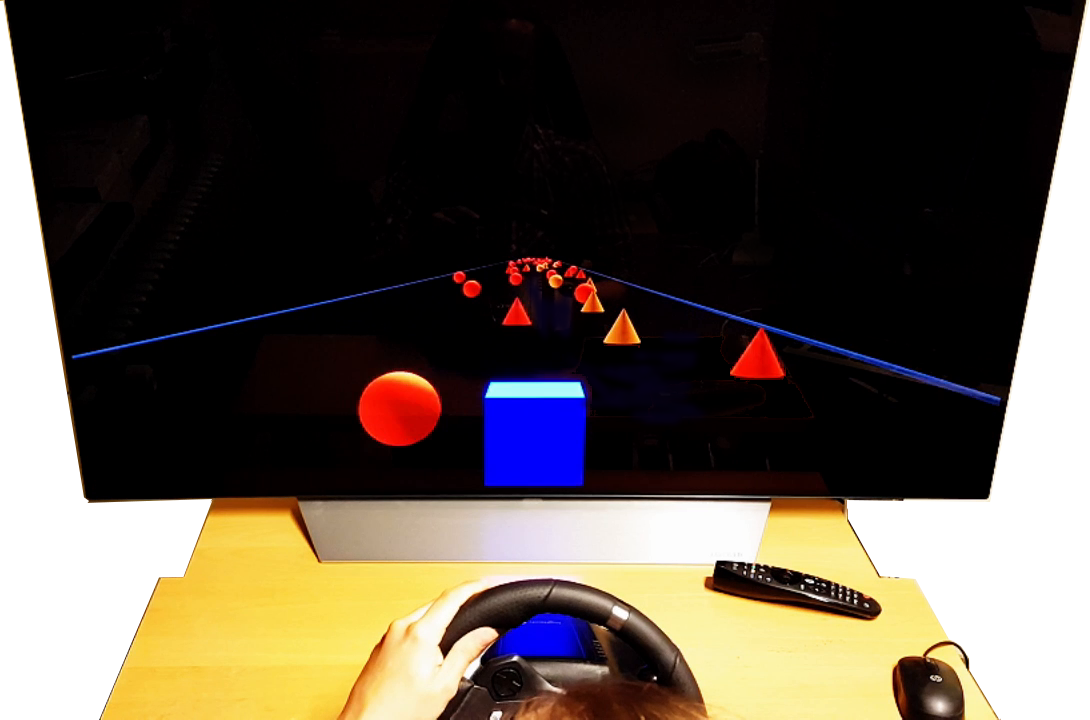
\includegraphics[width=\nicewidth]{Screenshot_cogcarsim}
	\caption{The high-speed steering task. The participant steers the blue cube to avoid conical/spherical obstacles on the track, which is bounded to each side by dark blue parallel lines. The game was designed to continually adapt the difficulty level (speed) to the participant's skill (obstacle collisions). Such balance is considered one of the key antecedents of Flow.}
	\label{fig:cogcarsim}
\end{figure*}

Nine participants (6M, 3F) played the game in eight sessions over a period of 2-3 weeks, one session per day, 5 trials per session (i.e. a total of forty trials, each about 2-4 min duration, depending on performance). Based on extensive informal piloting, we judged that the resulting about 2h would be sufficient to achieve good proficiency in this task, but with no ceiling effect. The 10 item Flow Short Scale \cite{Engeser2008} was filled after each trial to probe self-reported Flow in the task. Physiological data were recorded, during task and five minutes of baseline, in sessions one and five-to-eight.

This design allowed us to explore the following Research Questions:
\begin{enumerate}
	\item RQ1. How does performance change over time, i.e. what is the shape of the `learning curve' (LC)? Specifically, does performance in the game improve, and does improvement follow a power law of practice (as found in much previous work on visuomotor skill acquisition \cite{Newell1982})?

	\item RQ2. How is trial-wise self-reported Flow (from here on simply `Flow') related to performance? Specifically, is performance improvement across the whole experiment (i.e. learning) accompanied by higher levels of Flow?

	\item RQ3. Are there identifiable physiological markers of Flow and/or physiological measures that are predictive of task performance? Specifically, given its putative association with striatal dopamine\cite{Slagter2012}, spontaneous eye blink rate (sEBR) was of interest in our reinforcement-based learning task (positive reinforcement from increase in speed, negative reinforcement from collisions). Other measures were collected as well, but will be analysed and reported elsewhere; here we focus on the sEBR results.

\end{enumerate}

\section*{Results}
% We should aim to make results understandable without the detailed methods which will be placed at the end
All participants completed the task (40 trials in total). Average trial duration was 186s (SD 18.2s, min 162.2s, max 300.1s). Average number of collisions was 17.8 (SD 4.9, min 5, max 40). Average trial velocity ranged between 1.37 and 2.54 units per step (mean 2.23, sd 0.19). Maximum instantaneous speed was 3.6 and minimum 1.06. The supplementary information provides comprehensive data on performance-related features, such as trial duration, along with correlations between them (Fig.~\ref{fig:scatter_matrix}). For all results, detailed descriptions of statistical methods can be found in the Methods section.

\subsection*{RQ1: How does performance change over time?}

What is the form of the learning curve, does it consistently improve e.g. as a power law of practice \cite{Newell1982}? A power-law curve transformed to log-space will be linear. Thus, to investigate whether participant behaviour follows a power law, we fitted a linear model in log-log space (log-transformed dependent and independent variable) of trial durations as a function of cumulative number of trials, for each participant separately. Fig.~\ref{fig:flowVperf} (panel A) shows this log-log performance data for each participant in each trial. Blue dashed lines indicate the power-law LC. Distance of points from the line (residuals) indicate the deviation of each trial from predicted learning: points above the line indicate longer duration (worse performance) than predicted by the LC, and vice versa.

\begin{figure*}[!p]
	\centering
	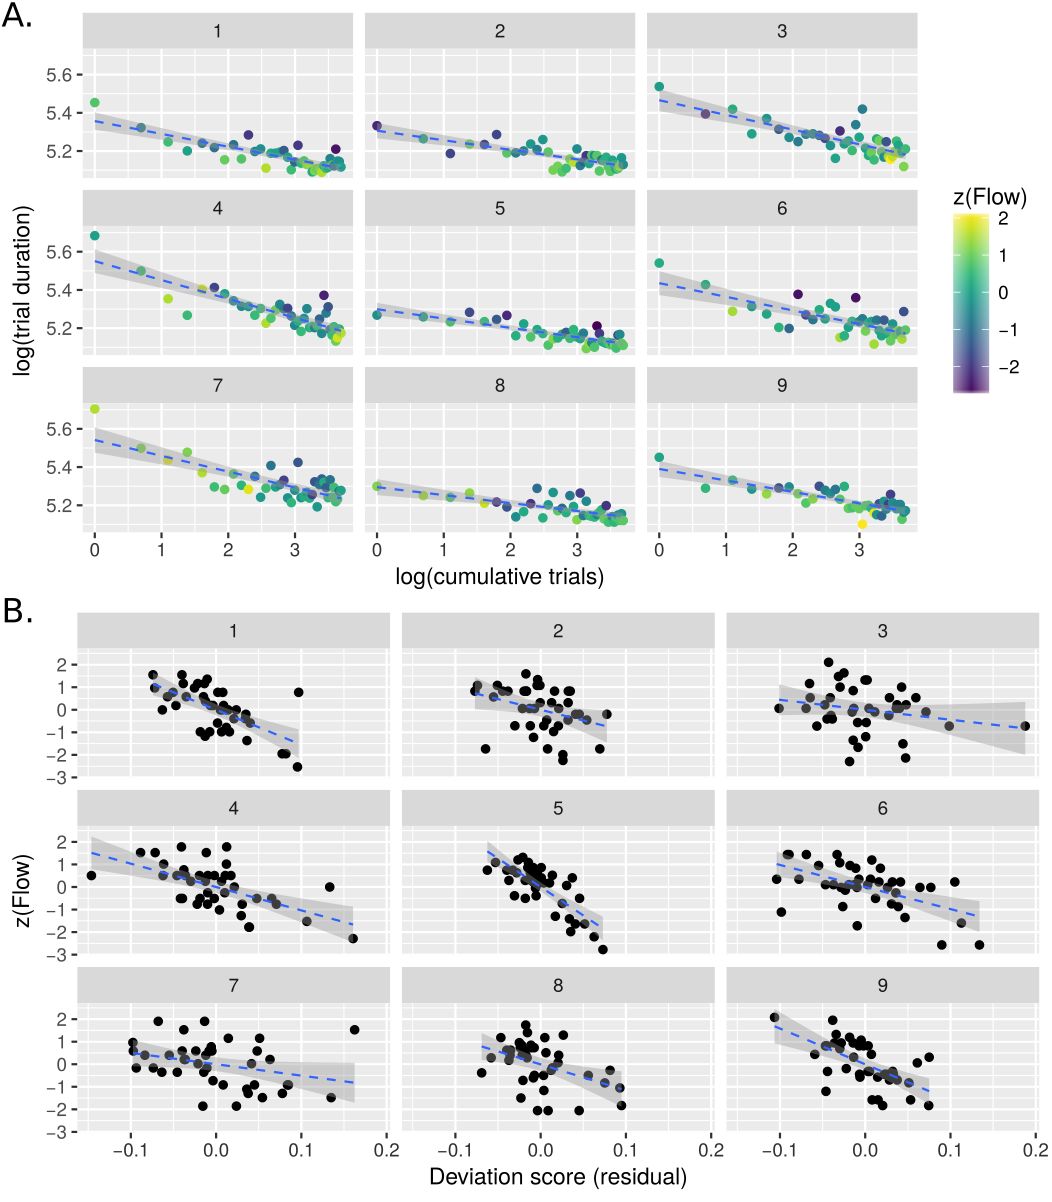
\includegraphics[width=\linewidth]{cogcar_main_anon}
  % \includegraphics[width=\linewidth]{flowDeviation_panelsRL3}
	\caption{{\it Panel A}: Participant-wise data showing logarithm-transformed performance and Flow self-reports in the speeded steering task. Ordinate shows log-duration of trials, abscissa shows log-cumulative trial count. Dashed blue lines fitted to the data are power-law learning curves, which transform to linear in log-log space.\\
  {\it Panel B}: Participant-wise deviation scores (observed trial duration minus predicted trial duration) plotted against Flow scores for each participant, and fitted by linear models.}
	\label{fig:flowVperf}
\end{figure*}

All participant-specific log-log models had negative slopes, which indicates that with experience each participant learned to play better (obtained faster trial times). The variation in intercepts reflects disparity in participants’ initial skill levels, and the variation in slopes the different learning rates. The individual intercepts and slopes of the models are presented in Table~\ref{tab:LCxFlow}. A grand model was also fitted for all participants, and cumulative number of trials explained 39.6\% of variance in trial durations. As the performance generally improves with cumulative trials, in agreement with a power-law of learning model, the explained variance can be ascribed to learning.

To confirm that a power law model gives a good approximation of learning, we compared its model-fit criterion against the fit of an exponential curve model (see Supplementary Information for details). While both models had good fit, the power law model was slightly better.

RQ1 can thus be answered: {\it the task was learned and the LC fit well to a power law model}. Given these positive answers, we may assume that the model provides a useful statistical estimate of performance expectation, i.e. how well the participants expect to perform can be estimated from the model.

\begin{table}[ht]
\centering
\caption{\label{tab:LCxFlow}Individual learning rate parameters (cols 2--4), Flow (cols 5--6) and perceived importance (P.I., cols 7--8) scores. Last row shows group-mean values of each column.}
\begin{tabular}{llllllll}
\hline
Participant & Intercept sec & Intercept log & Slope  & Flow mean & Flow SD & P.I. mean & P.I. SD \\
\hline
1           & 213     & 5.36      & -.067 & 5.10      & .51     & 3.53      & .57     \\
2           & 202     & 5.31      & -.049 & 5.18      & .39     & 4.29      & .47     \\
3           & 237     & 5.47      & -.077 & 5.36      & .64     & 2.03      & .50     \\
4           & 257     & 5.55      & -.099 & 4.40      & .39     & 4.12      & .46     \\
5           & 200     & 5.30      & -.049 & 5.44      & .88     & 5.16      & .64     \\
6           & 230     & 5.44      & -.071 & 5.22      & .82     & 4.33      & .56     \\
7           & 255     & 5.54      & -.083 & 4.69      & .53     & 2.22      & .53     \\
8           & 198     & 5.29      & -.041 & 4.94      & .90     & 3.67      & .70     \\
9           & 219     & 5.39      & -.059 & 5.25      & .79     & 4.62      & .55     \\
\hline
Group mean  & 223     & 5.41      & -.066 & 5.06      & .65    & 3.77      & .55    \\
\hline
\end{tabular}
\end{table}


\subsection*{RQ2: How is Flow related to performance?}

% data:  Flow and LC (from table 1)
% t = 2.0678, df = 7, p-value = 0.07747
% alternative hypothesis: true correlation is not equal to 0
% 95 percent confidence interval:
%  -0.08177327  0.90840927
% sample estimates:
%       cor
% 0.6157904
Participant-wise mean Flow and LC slope were related but not significantly correlated (Pearson's correlation coefficient {\it r} = 0.6, {\it p} = 0.9, N = 9). %NHST1
Since we have established that performance improves over sessions, we also used session number as a simple proxy of performance improvement. Fig.~\ref{fig:FlowVssn} shows the group-wise distribution of Flow scores plotted against sessions: clearly, there is no effect of session on group-wise median Flow (Pearson's {\it r} = -0.12, {\it p} = 1.0, N = 8).%NHST2

\begin{figure*}[!ht]
	\centering
	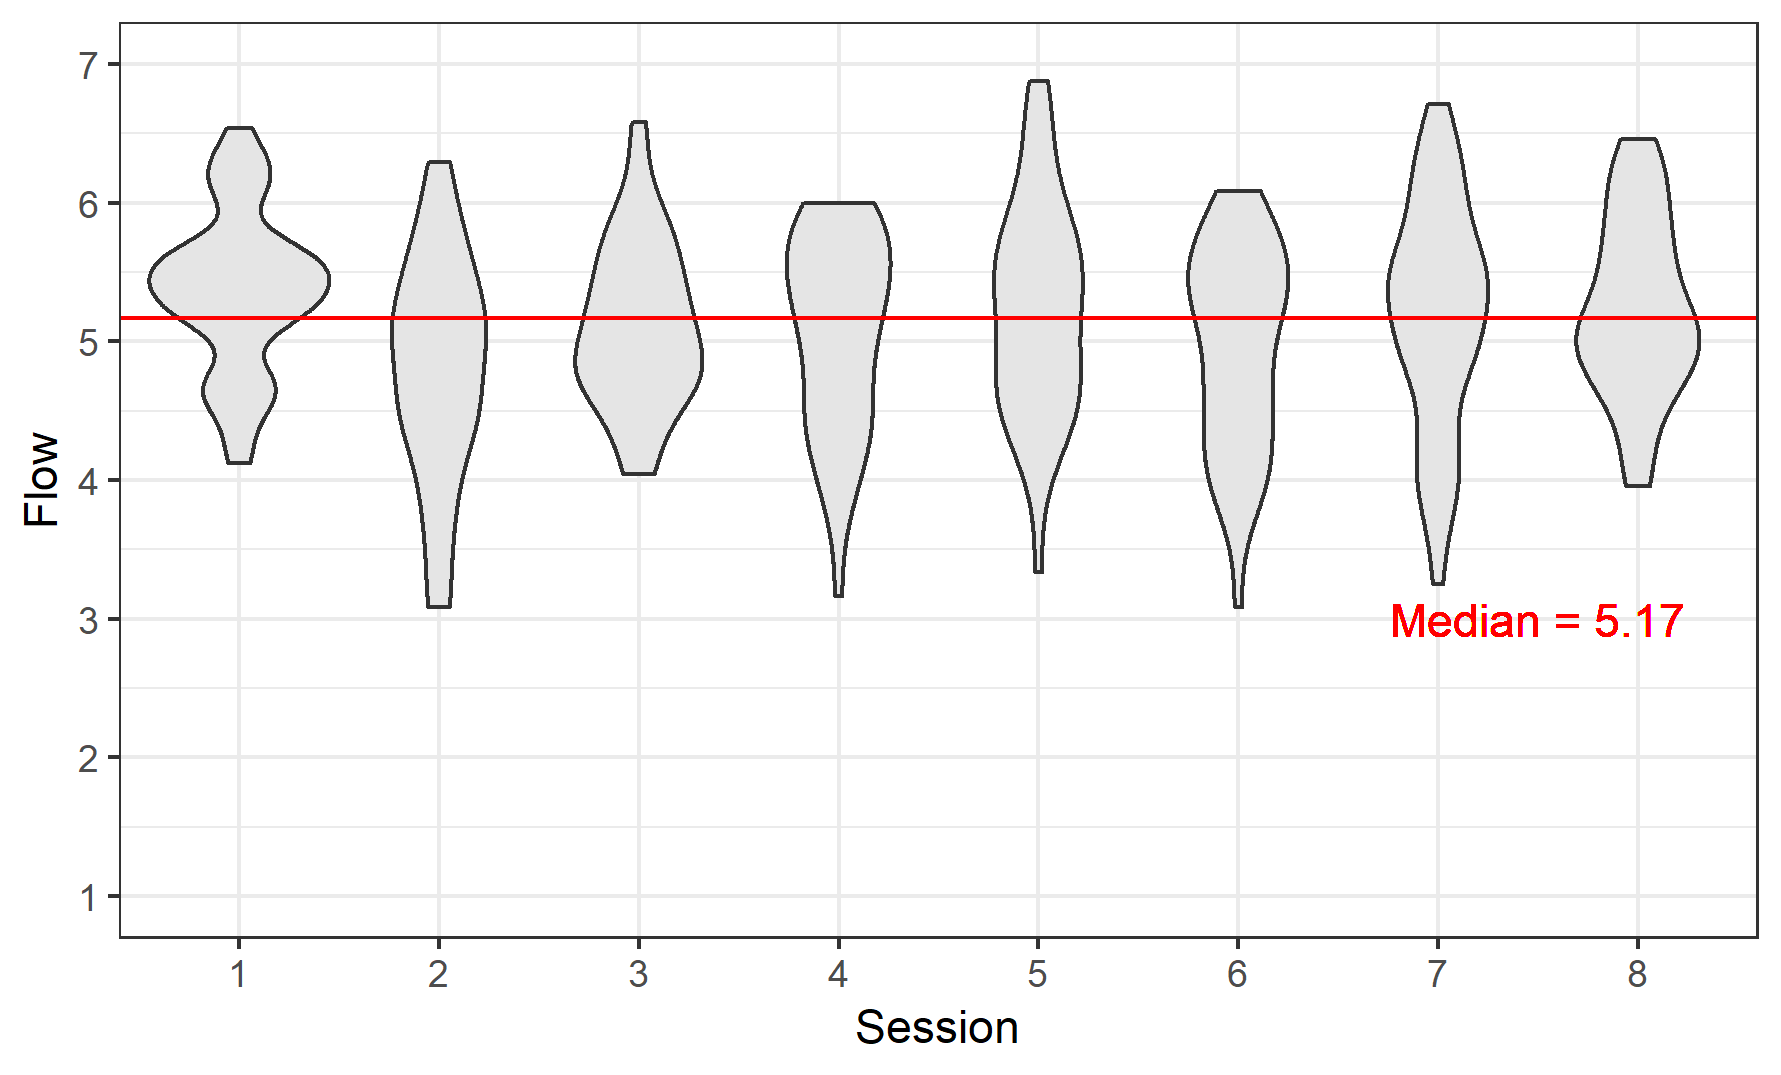
\includegraphics[width=\nicewidth]{session_fss2}
	\caption{Violin plot representing participants' self-reported Flow in sessions 1-8 (per-session Flow = mean of five trials. The self-report items are given in Supplementary information, the scale was 1-7).}
	\label{fig:FlowVssn}
\end{figure*}

Next, we calculated the group-wise correlation of median duration and median Flow, separately for each session. The relationship between duration and Flow was intermittently significant {\it before correction for multiple comparisons}, but not after, and with no particular trend (range of Pearson's {\it r} = [-.05 $\dots$ -.74], {\it p} = [0.3 $\dots$ 1.0], N=9 for all). These results suggest that higher Flow was sometimes associated with lower trial durations (i.e. better performance), but not strongly and not systematically. If we group sessions by condition (introduction=1, practice=2--4, main test=5--8), we can visualize the evolution of performance against Flow more clearly than by plotting each session individually, see Fig.~\ref{fig:FlowVdurXssn}.%NHST3-11

\begin{figure*}[!b]
  \centering
  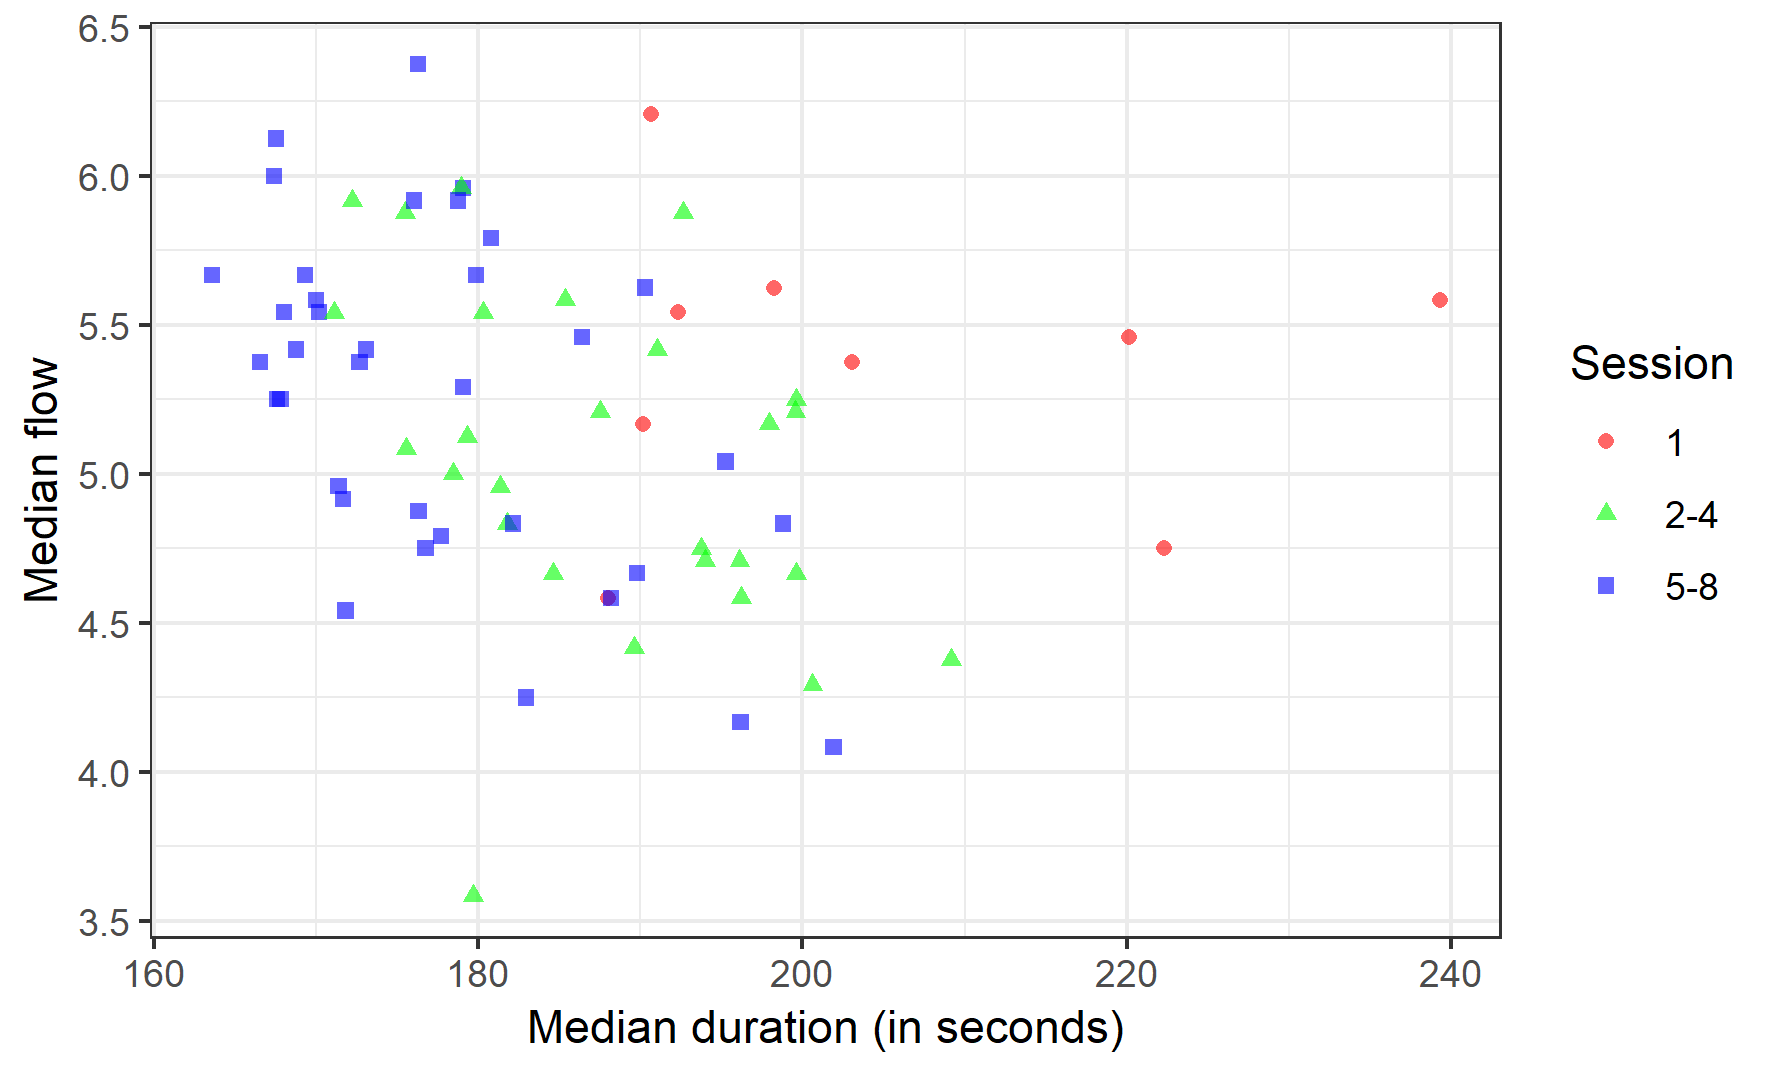
\includegraphics[width=\nicewidth]{session_flowDuration_v3}
  \caption{Duration and Flow over sessions grouped: 1, 2-4 (training), 5-8 (physiological measurements), N = 72.}
  \label{fig:FlowVdurXssn}
\end{figure*}

The relationships between global (over all responses) Flow and performance appear weak, but we also wish to examine local Flow for each trial separately. The points in each subplot of Fig.~\ref{fig:flowVperf} (panel A) are coloured according to Flow self-reports made after each trial, in a standardised range (original scores transformed to {\it z}-scores). The highest Flow scores are green, the lowest are red. Interestingly, this figure reveals at a glance that the points lie above and below the log-transformed power-law line in good agreement with the level of experienced Flow: worse performing trials (data-point above the line) tend to be more red (Flow scores below the participant-wise mean), and better performing trials tend to be more green (scores above the mean). In other words, it seems that whenever participants were performing {\it better than predicted by the power-law line}, they were experiencing more Flow, and {\it vice versa}.

We evaluated whether this effect was robust and statistically significant. For each participant, we correlated their {\it deviation scores} (signed residuals from the power-law model) with their Flow scores, using a linear mixed model (see Methods). This model was statistically significant (deviation score $\beta$ = -8, {\it t} = -4.36, {\it p} = .003) %NHST12
and the relationship is shown in Fig.~\ref{fig:flowVperf} (panel B; Flow scores are standardized). The conditional pseudo-$R^2$ value for this model was .47, corresponding to a correlation of ~.68, so that the model explains $\sim$47\% of Flow score variability.

Thus, {\it high Flow scores are associated with better than predicted results} (trial durations below the predicted performance line), and {\it vice versa}. The strength of this association per participant follows from the strength of the correlation, and overall the model has large effect size.

As can be seen in Fig.~\ref{fig:flowVperf} (panel B), the trend was clearly negative for 7 out of 9 participants, while for two participants, 3 and 7, the trend was similar but the relationship was weaker. Notably, these two participants also reported lower scores on perceived importance: mean scores for these participants were 2.03 and 2.22, whereas the overall mean was 3.77 (see Table ~\ref{tab:LCxFlow}). However, the group-wise interaction between perceived importance scores and deviation scores was not statistically significant.

RQ2 can thus be answered: Flow was not consistently and robustly related to improvement in task performance with the skill acquisition occurring over 2 h of practice. It was, however, consistently related to whether performance was {\it better (or worse) than predicted} given the participant LC. Moreover, this effect might be moderated by self-reported perceived importance of the steering task (more data would be required to clarify).

\subsection*{RQ3: Is spontaneous eye blink rate related to performance or Flow?}

sEBR showed a negative relationship to participant-wise LC slopes, as shown in Fig.~\ref{fig:EBRvLC}. The correlation is of moderate strength, though non-significant (Pearson's {\it r} = -.46 , {\it p} = 1.0, N = 9). %NHST13
The LC slope of every participant was negative, which means we can say that the smaller the sEBR, the shallower the LC slope. Or, because slope and intercept are highly correlated, it is almost equivalent to say that smaller sEBR correlates with better initial performance.

Mean Flow scores are not related to sEBR, as can be seen in Fig.~\ref{fig:EBRvLC} (Pearson's {\it r} = 0.15, {\it p} = 1.0, N = 9). %NHST14
However, examining the Flow scores in Fig.~\ref{fig:EBRvLC} turns up an interesting relationship: the residuals of the fitted linear model (i.e. vertical distance of each data-point from the line) are {\it strongly} related to mean Flow scores (Pearson's {\it r} = -.86 , {\it p} = .04, N = 9). %NHST15
In other words, participants' mean Flow scores are strongly correlated with their observed deviation from the modelled linear relationship between sEBR and task learning (LC slope). This correlation is not driven only by the non-significant correlation of Flow and LC (described above). In fact, interaction analysis (see Methods) shows that when Flow mean is above 5.05, LC slope significantly predicts sEBR at {\it p} $<$ 0.0001.
%%%% FLOW X SEBR COR TEST
% data:  FM and sEBR
% t = 0.41014, df = 7, p-value = 0.694
% alternative hypothesis: true correlation is not equal to 0
% 95 percent confidence interval:
%  -0.5688016  0.7418380
% sample estimates:
%      cor
% 0.153187

%%%% FLOW X RESIDUAL COR TEST
% data:  FM and abs(LC - LM$fitted.values)
% t = -4.4556, df = 7, p-value = 0.002952
% alternative hypothesis: true correlation is not equal to 0
% 95 percent confidence interval:
%  -0.9700331 -0.4562393
% sample estimates:
%       cor
% -0.859833

\begin{figure*}[!ht]
	\centering
	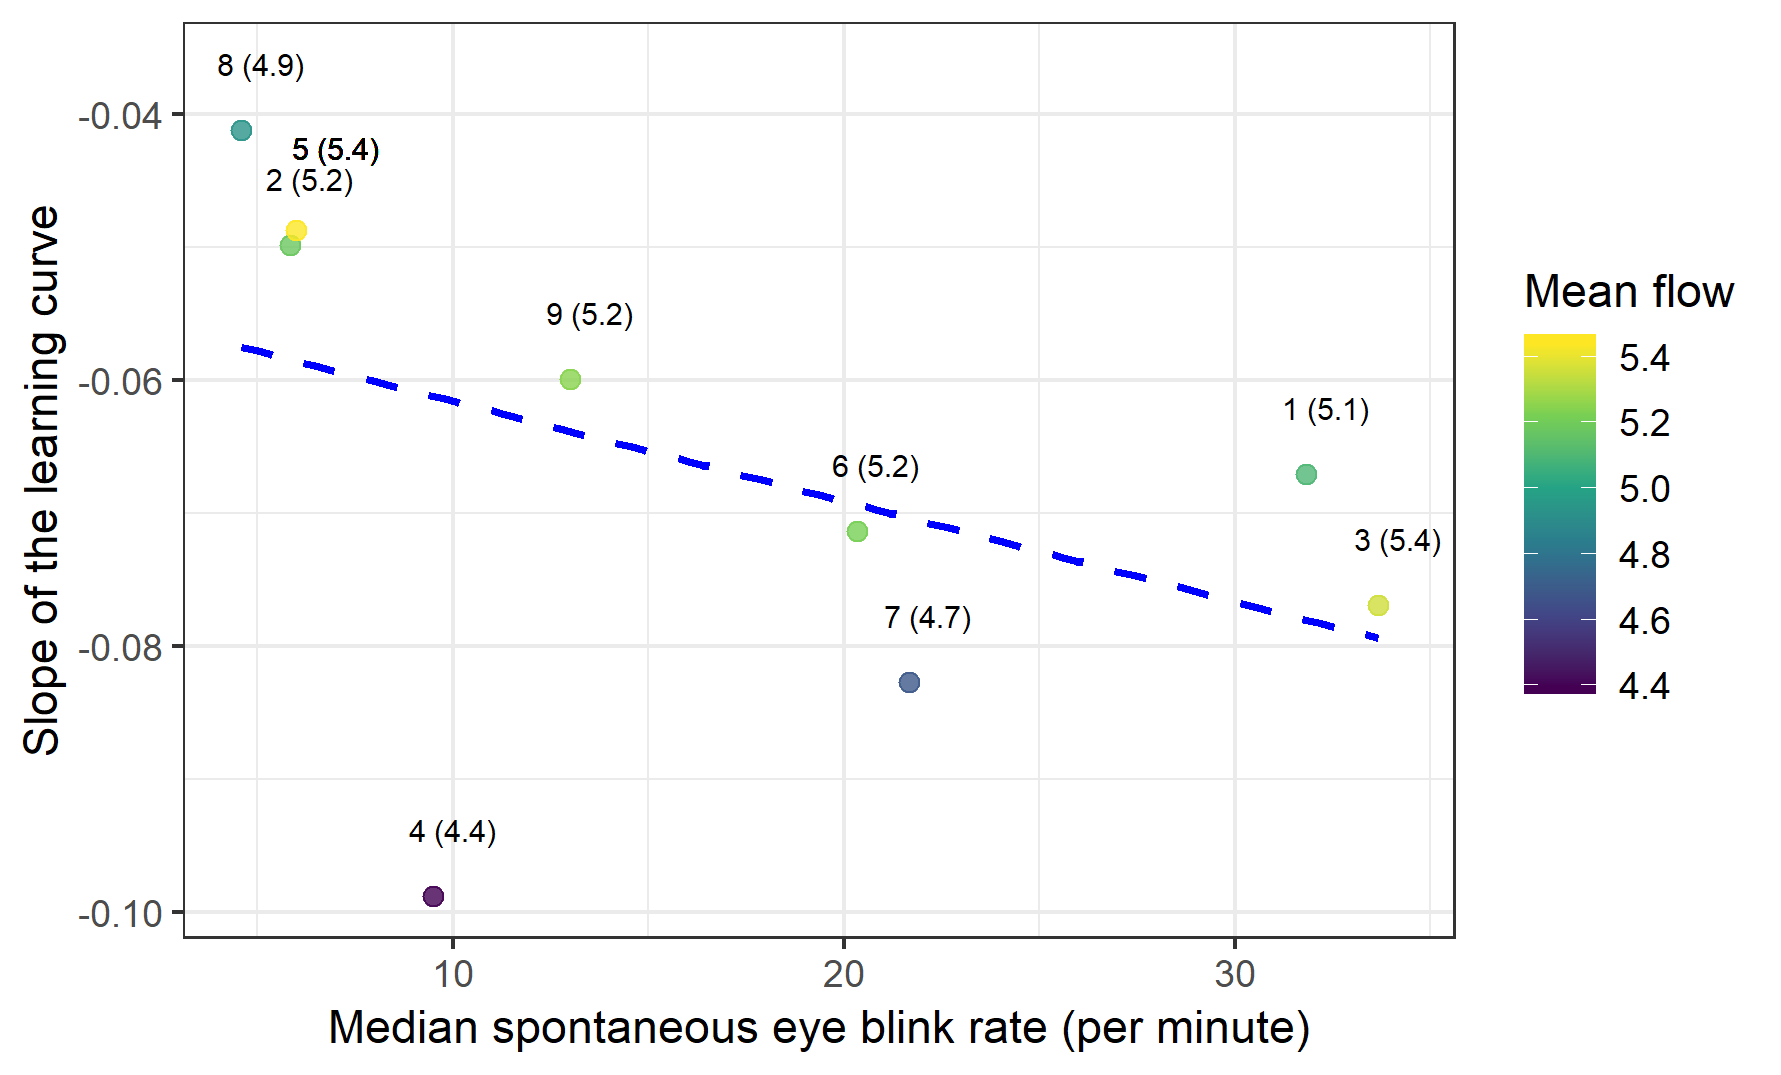
\includegraphics[width=\nicewidth]{lcurve_sbr_flowRL2}
	\caption{Participants' median spontaneous eye blink rate plotted against the slope of their learning curve, and coloured by their mean Flow scores. Linear model is depicted by the dashed line. Each point is labelled with the participant number (1..9) and exact mean Flow score (in parentheses).}
	\label{fig:EBRvLC}
\end{figure*}


%%%%%%%%%%%%%%%%%%%%%%%%%%%%%%%%%%%%%%%%%%%%%%%%%%%%%%%%%%%%%%%%%%%%%%%%%%%%%%%%
%%%%%%%%%%%%%%%%%%%%%%%%%%%%%%%%%%%%%%%%%%%%%%%%%%%%%%%%%%%%%%%%%%%%%%%%%%%%%%%%
%%%%%%%%%%%%%%%%%%%%%%%%     DISCUSSION    %%%%%%%%%%%%%%%%%%%%%%%%%%%%%%%%%%%%%
\section*{Discussion}
% exploration of Flow and on-task learning (LC as opposed to pre- post)
We present a longitudinal experiment of Flow in a game-like high-speed steering task where task performance is easily parametrised and its relation to Flow and sEBR analysed. % game was fairly successful in eliciting Flow-like experiences (high baseline, score five out of seven)
To induce Flow, the game was designed to hold the balance between skill and challenge constant: the difficulty of the game continually adapted to the skill level of the participant.

The results show the game was clearly Flow-inducing: `baseline' average Flow across sessions was reported as 5.1 (out of 7) on the FSS. %we do not see Flow increasing as you learn the game; it is not that when you play better you get more Flow
We further found that Flow was not associated with gaining experience and skill in the game -- our participants did not reliably report more Flow even as they learned, session by session, to complete the trials faster. These results support the theoretical position (e.g. as per \cite{Keller2012}) that Flow is elicited by the balance of skill and challenge, but show that Flow is less sensitive to the absolute level (within a task) of skill or challenge.

% we are relating Flow to the learning mechanisms: the Flow reports across time are related via the LC (skill level)
% we do see that when you play better than expected, you report more Flow (but caution: direction on causation between Flow and performance unclear - does Flow lead to better performance or does better performance lead to higher (post hoc) self-reported Flow?)
Moreover, higher `local' Flow (trials with higher self-reported Flow) was associated with trial durations shorter than expected by the power law LC model. In other words, while global average Flow remained relatively high and stable across all sessions, higher-than-average or lower-than-average Flow was associated with performance that was better or worse than expected (at the current level of skill).

In other words, learning to play the game did not itself increase Flow; rather, the game induced a fairly high level of `baseline' Flow, and local variability around this baseline was correlated with better or worse than statistically-expected performance. The relatively stable Flow baseline induced by the game could be construed as reflecting the meeting of skill and challenge {\sf C1--3} by design.

It is a novel observation that local Flow relates to fluctuations of performance around the level expected from the learning curve. It is interesting because higher-than-expected performance in an individual trial can plausibly indicate either higher skill (e.g. better concentration), or lower challenge (easier-to-negotiate random placement of obstacles). Both are deviations from the average skill-challenge balance, yet may be associated with higher Flow.

Why is this? One possibility is that performance on some trials is enhanced by increased Flow during the trial - i.e. participants perform better when they ``get into Flow''. Another possibility is that the randomly-generated geometric layout of each trial might be more or less easy to negotiate. If this is so, and if on average the skill-challenge balance in our task is slightly on the challenging side, then the `easier' trials would both afford faster performance and also bring the task closer to the optimum balance of skill and task demand. Alternatively, participants may be more likely to report higher Flow (after the fact) on a more successful (hence, more rewarding) trial, because they see their score before they complete the FSS. These alternatives cannot be readily discriminated in the present paradigm (though the first two seem most plausible, see Limitations below).


\subsection*{Learning, Flow, and models}
% Relation to previous Work on skill acquisition and Flow
How can our approach and the present results be helpful to understand the mechanisms generating the Flow experience?

% it's a good idea to look at Flow in relation to skill, across points in time...because we want to understand the mechanisms generating the experience (and the report of the experience)
Methodologically, this study follows a {\it time series} approach little used in Flow research, by looking at changes in Flow over time, with relatively highly frequent and non-independent repeated measurements. This contrasts with much prior work which treats Flow as a relatively stable property.

One contribution of our study is how, due to the novelty of the approach, it helps shed light on theoretical models of Flow. Psychological theory of Flow has dealt mainly with state and trait models \cite{Csikszentmihalyi1975}, and recent conceptual Flow research \cite{Moneta2012} has critically examined the classic octant/quadrant models \cite{Massimini1988}. Related work by Keller and Landh\"{a}usser proposed an update \cite[pp-56]{Keller2012}: the Flow intensity model, which focuses on {\it perception} of challenge--skill balance and of task importance as governing factors for Flow. However, our study highlights the need to look not just at Flow experience, but at the (evolving) cognitive process that generates the experience, which is also related to {\it on-task} learning and skill acquisition.

To see this, consider our experimental performance data through the lens of either the Flow quadrant/octant model, or the Flow intensity model: they lead us to expect that as skills improve and challenges are consequently raised then Flow self-report should increase over time. Learning implies skill increase, which (by game design) implies challenge increase, which (by model design) together imply Flow increase.

Specifically, in the octant/quadrant model, if skills and challenges increase, the individual should feel further `north-east' of the median point where Flow bottoms out, and thus be more likely to report Flow and assign it greater intensity on a reporting scale. In the Flow intensity model, increased skills should increase both perceived fit of skills and task demands (because skill-learning increases access to the task's deeper levels of challenge); {\it and} subjective value of the activity (because skill-learning can increase the learner's investment in the task). In summary, for such `state Flow' models' the reference frame is fixed, leading to the prediction of increased Flow with skill acquisition. This is not supported by our data, and it is thus not straightforward to reason about the evolution of Flow, or learning and Flow, based on these models.

Regarding Flow as a dynamic process means it must be bounded, since human psychological processes should be homeostatic (e.g. have no positive feedback loops) to remain viable. Then, the natural homeostatic quality of a bounded dynamic process will tend to maintain Flow self-report at a level proportionate to the temporally local self-concept of skills and challenges. This does agree with our data, but there is less theoretical work available on which to base such a cognitive information-processing view of Flow.

Prior art has provided some (neuro)cognitive, information-processing work on Flow: including Marr's biobehavioural model \cite{Marr2001}; this lead author's model, which integrated elements from information theory to neurobiology \cite{Cowley2008}; or more recently, a descriptive model proposed by {\v{S}}imle{\v{s}}a and colleagues \cite{Simlesa2018} using a combustion-engine metaphor. Such conceptual work could provide an approach to make cognitive hypotheses about Flow, but these models were never empirically tested, so it is unclear which (if any) to follow.

% Without aiming to propose a new model here, we can, based on our behavioural data, consider Flow and learning
A possibly more novel way to view Flow and learning is via task complexity. Flow has been proposed to be possible in {\it any} task, complex (e.g. car driving) or simple (e.g. dish washing) \cite{Csikszentmihalyi1999}, but has also been proposed to depend on perceived task importance and a sufficient level of challenge \cite{Keller2012}. One way to resolve these ideas is to consider that the individual can {\it introduce} complexity to their activity if they appear to have exhausted a task's potential to challenge them. Nakamura and Csikszentmihalyi \cite{Nakamura2002} suggest such an exploratory mechanism to explain how individuals maintain Flow in complex tasks: ``As people master challenges in an activity...to continue experiencing flow, they must identify and engage progressively more complex challenges.'' The corollary for simple tasks is that individuals {\it create} complexity, e.g. with self-defined goals \cite{Rauterberg1995}. For example, a similar state to Flow, called the Zone, has been reported for machine-gambling addicts whose pastime is in fact skill-free, but who nevertheless believe that they are skilled \cite{Schull2014}.

In other words, complex tasks have deep structure to be learned, requiring non-trivial skill acquisition for any duration of learning and thus a shallow LC (learning is slow). Importantly, the skill level does not quickly peak, such as with simpler tasks like washing the dishes, where Flow might be obtained but cannot strongly interact with learning (without self-created complexity). Learning comes into play when we consider that the same task can appear at first simple and later complex, e.g. as our experiment game.

This distinction can help us reason about Flow processes by considering separately the complex types of cognitive tasks (when they elicit Flow), which we label as {\bf high performance cognition (HPC)}. The aim of future work should then be to find out: what cognitive processes are {\it specific} to HPC (in different stages of learning), but also {\it general} to multiple performance-domains? By so doing, we can in future attempt to clarify empirical observations by reference to a distinct cognitive theory of how Flow is generated -- i.e. HPC theory.


% Relation to previous Work on eye blink rate
\subsection*{Learning, Flow, and sEBR}
Our evidence suggests a clear linear trend relating sEBR and LCs (Fig.~\ref{fig:EBRvLC}): the larger the sEBR, the steeper the LC slope (or: the higher the LC intercept). The distance of data-points from the fitted model values also closely match the distribution of Flow mean scores, meaning that individuals with lowest Flow also diverge the most from the sEBR$\times$LC model. Interaction analysis then supports the idea that sEBR correlation with LC is stronger the higher the global Flow. We thus claim that there is a genuine sEBR--LC relationship that is moderated by Flow. This brings to the fore the issues of underlying mechanisms and causality. We cannot decide causality based on our data, but there is literature relevant to mechanisms, that can help identify future directions of inquiry.

Learning is influenced by the context-dependent disposition of the learner, which is to say learning is governed by psychological factors (motivation, prior experience), but also physio-/neurological factors. One relevant factor is the well-established relationship between attention and striatal dopamine levels \cite{Dreisbach2005}. The striatum plays a major role in decision making and reward/aversion processing, moderated by the level of tonic dopamine D2-receptors therein; dopamine imbalance can thus bias the entire learning process. This is illustrated for example in studies of `attentional blink' (AB) by Slagter and others \cite{Slagter2012,COLZATO2008}), which suggest a U-shaped function between tonic striatal dopamine and AB size. In other words, excess or insufficient dopamine D2-receptor density can impair attention via too rapid (distractible) or too slow (inattentive) attention updating.

sEBR has been suggested as an externally-measurable index of striatal dopamine level (though caution is needed, see Dang {\it et al} \cite{dang2017spontaneous}). Early work by Karson \cite{Karson1983} linked sEBR to striatal dopamine in humans and other primates. Taylor and colleagues \cite{Taylor1999} then localised to the caudate nucleus, whose normal function is implicated in classification learning \cite{Seger2005}; caudate nucleus volumetric asymmetry is implicated in inattention symptomatology \cite{Schrimsher2002}. Later work from Slagter \cite{Slagter2015} has shown that sEBRs may relate specifically to avoidance learning; others have linked dopamine levels and sEBR to perseverance, distractibility and cognitive control \cite{Muller2007,Dreisbach2005}. Finally, DeManzano {\it et al} \cite{DeManzano2013} have shown that  predisposition to experience Flow is positively correlated with striatal dopamine D2-receptor availability, specifically in caudate and putamen, and always stronger in right hemisphere than left.

Let us consider learning as a process whereby perception, cognition and action become attuned to task demands. In our game task, learning involves high-frequency decision making with respect to continuously updating stimuli of uniform kind (not unlike AB task, a continuous performance test designed to probe AB size \cite{Slagter2012}). In this view (proposed for focus, not to deny all other options), the sEBR--LC relationship could be interpreted as showing that higher sEBR supports learning. The underlying mechanism could be that higher dopamine levels permit more rapid attention updating and thus more fluid response to changing task demands. This can work despite Slagter {\it et al}'s \cite{Slagter2012} proposed U-shaped function: because our game-task constantly maintains a level of demand slightly greater than the participants' skill. Thus, in this context, higher sEBR tends to be better, possibly because the {\it requirement} for rapid attention updating grows with the learned task skill.

Flow was reduced in those participants who deviated (positively or negatively) from this relationship. Lower Flow could be due to, e.g., misalignment of task demands and attentional updating rate, creating a more effortful experience. So the observed moderation by Flow scores of the sEBR--LC relationship could be explained by neurophysiological difficulty of adjusting attention updating in response to changing task speeds. In other words, it may not be the case that an absolute level of striatal dopamine should predict learning, but rather an individual level relative to how each participant relates to the task (vis-\'{a}-vis gaming experience, motivation, fine motor skills, or potentially many other variables). If a participant's tonic dopamine is not at their ideal level for this task, they might nevertheless do well in the task, and yet find the experience more effortful and less fluid (than is suggested as Flow-like by wording of the FSS).


\subsection*{Limitations and Future Work}
Our study had a small convenience sample because (a) the recording paradigm was extensive (around eight hours of contact time), and (b) it was to some degree an exploratory study; both implying the need to constrain datasets to tractable sizes. Regardless of the justification, the sample size and method are limitations to be remedied in future work. Additionally, lacking experimental manipulations the study cannot make strong causal claims, which could be improved by recording separate conditions of the game task, e.g. with varied difficulty levels.

As stated above, there are different plausible explanations of the main result linking Flow and performance. If FSS reports were indeed influenced by seeing the score beforehand, this could be considered a drawback. However, the game gives such clear and direct feedback on performance (i.e. after collisions), that it is likely that self-assessment of performance would be similar with or without seeing the score. The score can thus be considered just a reinforcement of the perceived fit of skills and demands, which is anyway a required part of Flow reporting \cite{Keller2012}.

Trial-by-trial analysis is limited by the Flow self-report which only has one datapoint per trial. It would be more powerful to analyse {\it inside} each trial. In our data, self-reported Flow is a point model of an entire trial, for which the participant knows their score. Self-reported Flow is thus an after-the-fact report, and could be criticized for not capturing the in-the-moment {\it experience of Flow}, which might fluctuate greatly during a trial. Analysing the fluctuation of Flow-experience requires us to model individual actions and/or their outcomes, and sample Flow during performance. This is a difficult challenge, because paying attention to one's phenomenal state might easily disrupt the very processes sustaining that state, especially for Flow which is unreflective by definition. Future work should aim to model the conditions of Flow ({\sf C1--3}) in real-time, while simultaneously recording participant physiology, to uncover in greater detail the relationships involved. The existing dataset will be used for this purpose, in a pending report on the biosignals recorded with high temporal resolution, primarily electro-dermal activity.

To further explore the possible role of striatal dopamine, it would be interesting to experimentally manipulate the game to adjust the distance between obstacles, thus altering the attention-updating rate required to navigate without collisions (motor precision variation can be minimised by a suitably long training period). This manipulation could be varied in response to measurements of sEBR (which can be automated, e.g. by using electro-oculography \cite{toivanen2014}), to systematically investigate whether sEBR holds explanatory power with respect to individual variability in learning.


\subsection*{Conclusion}

% We report results that show how Flow assessment relates to the local reference frame provided by LCs; with evidence that the LC across sessions is predicted by participants' spontaneous blink rate.
We report results that self-reported Flow in a novel, challenging, and engaging high-speed steering task relates to trial-by-trial task performance relative to the learning curve: `better than expected' trials have higher Flow scores, and `worse than expected' trials have lower scores. The average level of self-reported Flow was high, as the game was specifically designed to meet the main preconditions of Flow, including balance of current skill and challenge. Perhaps surprisingly, Flow did not seem to change with global skill development or improvement in task performance.

We also report evidence that slope of the learning curve (total play time about 2 h, distributed over two weeks) is predicted by the participants' spontaneous blink rate, moderated by global Flow. This relationship potentially indicates a role for striatal dopamine in learning the visuomotor steering task, which may also relate to the experience of Flow as a response to felt attentional effort.


%%%%%%%%%%%%%%%%%%%%%%%%%%%%%%%%%%%%%%%%%%%%%%%%%%%%%%%%%%%%%%%%%%%%%%%%%%%%%%%%
%%%%%%%%%%%%%%%%%%%%%%%%%%%%%%%%%%%%%%%%%%%%%%%%%%%%%%%%%%%%%%%%%%%%%%%%%%%%%%%%
%%%%%%%%%%%%%%%%%%%%%%%%%%    METHODS    %%%%%%%%%%%%%%%%%%%%%%%%%%%%%%%%%%%%%%%
\section*{Methods}
\subsection*{Participants}
A convenience sample (N=9, 6 males, 3 females) was recruited via student mailing lists at the University of Helsinki, as well as personal contacts. The participants were between 22-38 years of age (mean 27, SD 3) with normal or corrected-to-normal visual acuity and no history of neurological or psychiatric disease.

\begin{table}[ht]
\centering
\caption{\label{tab:Participants}Participant background information.}
\begin{tabular}{lllll}
\hline
Participant & Gender & Driving license & Driving experience (km) & Gaming experience \\
\hline
1 & M & yes & 1,000-10,000 & At least one hour a week \\
2 & M & yes & 10,000-30,000 & At least one hour a week \\
3 & F & no & 0-1,000 & None or very little \\
4 & F & yes & 0-1,000 & At least one hour a week \\
5 & M & yes & 30,000-100,000 & At least one hour a week \\
6 & M & yes & 30,000-100,000 & 1-3 hours a month \\
7 & F & yes & 10,000-30,000 & None or very little \\
8 & M & yes & 100,000+ & 1-3 hours a month \\
9 & M & yes & 10,000-30,000 & At least one hour a week \\
\hline
\end{tabular}
\end{table}

Eight of the participants had a driving license; two participants reported $<$ 10,000 km lifetime kilometrage, three
participants 10,000-30,000 km, two 30,000-100,000 km, and one participant $>$ 100,000
km. Two had no or very little previous gaming experience, two participants played 1-3 hours a month, and five participants stated they play over one hour a week.

All participants were unaware of the purpose of the study, other than that the time of recruiting they were informed that the experiment was about game experience and learning. Participants were given 11 cultural vouchers (1 voucher is worth 5€) in compensation for their time. They were told that they would get 9 vouchers for participating in all sessions and 2 extra vouchers if they improved their performance in the game. The criteria for sufficient improvement were not stated explicitly, and in fact all participants were given the two extra vouchers.

\subsection*{Design}
The experiment was divided into eight sessions, on eight different days over a period of 2-3 weeks scheduled at each participant's convenience. In each session, the participant played five trials of the driving game, each trial lasting 2-4 min depending on their performance, for approximately 15 min of driving time per session. After each trial, the participant was shown the trial duration and the number of collisions, after which they filled in a self-report questionnaire (FSS). In sessions 1 and 5-8 (lasting approx. an hour), physiological signals were measured in a 5 minutes baseline recording before playing, and during gameplay. In sessions 2-4 (lasting 20 to 30 minutes), no physiological measurements were taken.

\begin{figure*}[!ht]
\centering
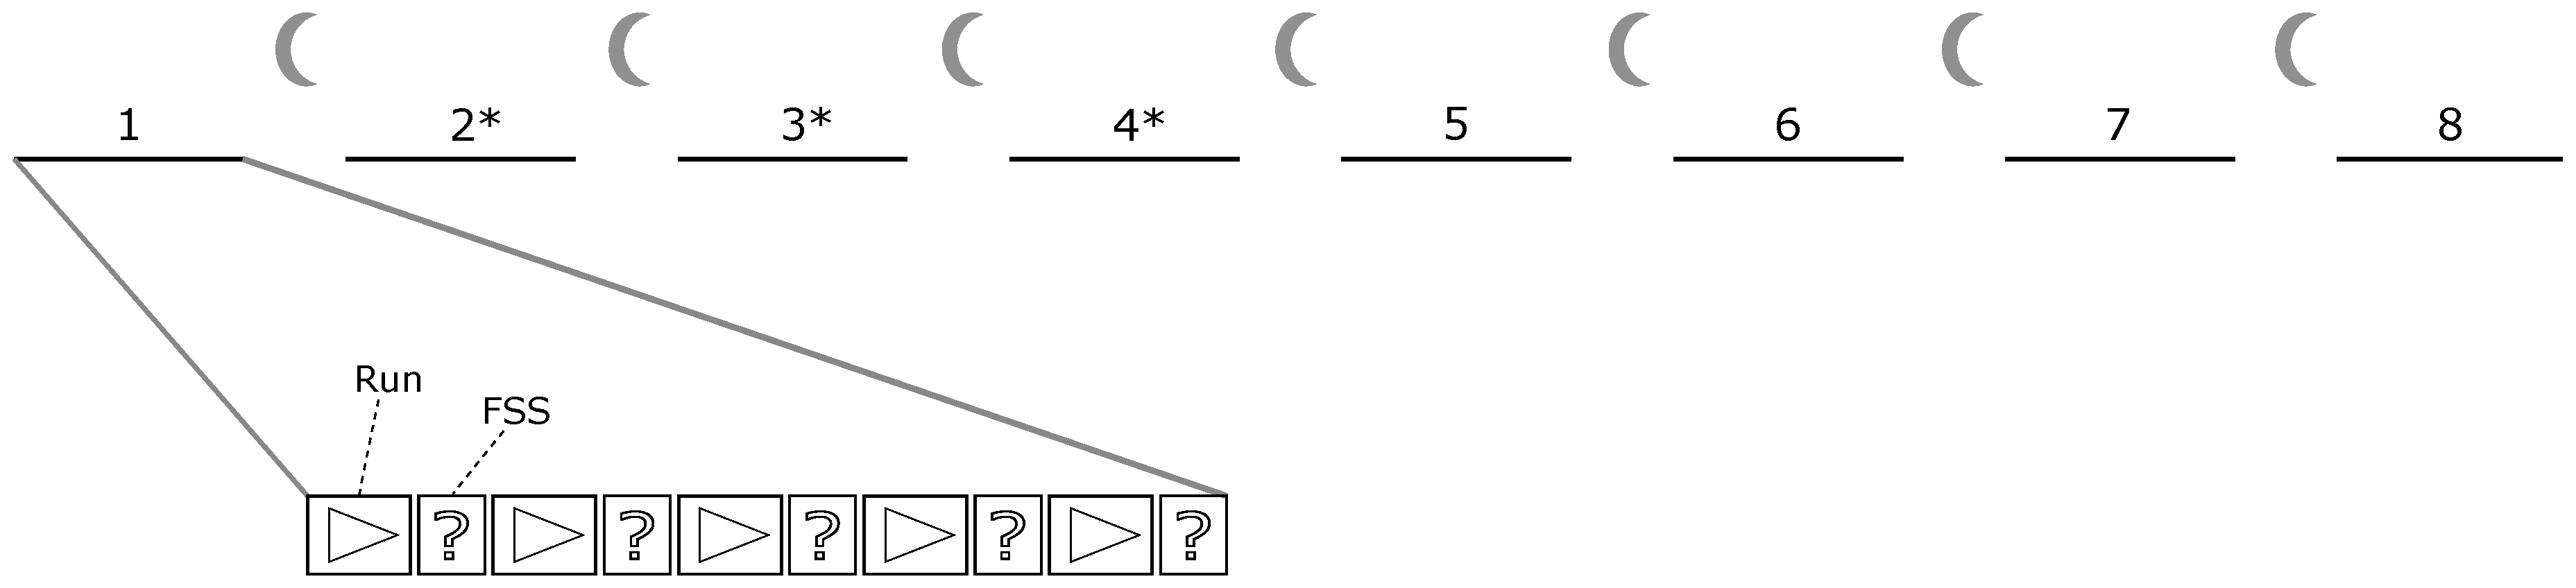
\includegraphics[width=\nicewidth]{design1}
\caption{The game was played in eight sessions on eight different days. In sessions 1 and 5--8, physiological signals were recorded during task performance; in sessions 2-4(*) no physiology was recorded. Each session consisted of five trials (2 to 4 min) followed by a self-report questionnaire (FSS, Flow Short Scale) about the latest trial.}
\label{fig:design}
\end{figure*}

\subsection*{Materials}
\paragraph{Game.} The experimental task was a custom-made high-speed steering game {\it CogCarSim} designed specifically (by OL and JV) for the study of Flow and coded in Python (by JV). The game code as used herein is permanently available under open source licence at \url{https://doi.org/10.6084/m9.figshare.7269467}.

The participant steered a cube `avatar' moving forward along a straight track bounded by edges that could not be crossed. The cube's side length was 2 units, and the track was 25 units wide.  The horizontal field of view angle of the virtual camera was 60 degrees and vertical 32 degrees. The camera was positioned behind the cube at 4 units height, pointing forward along the track.

Stationary obstacles (red cones, red or yellow spheres with a height/diameter of 2 units) on the track had to be avoided. For each trial, a total of 2,000 obstacles were placed randomly on the track, with placement constrained to always allow a path through. Track length varied between 24196.4 and 24199.7 units (mean 24197.8, sd 0.8). The speed of the cube was initially set to 1.6 units per step (96 units per second); increased at a constant rate (0.0012 units/step at every step); and slowed down if obstacles were hit (0.102 units/step at each collision). When a collision caused a speed drop, the screen flashed to indicate a collision; there followed an immunity period of 100 steps during which additional collisions did not cause further speed drops. Participants could only affect speed indirectly, by avoiding collisions.  Participants were instructed to avoid as many obstacles they could in order to complete the trial as fast as possible.
% Speed was not directly controlled by the participant, but instead increased linearly - starting each trial from a predefined velocity of 1.6 units per step. Colliding with obstacles slowed the speed down by a constant increment (0.102 units), and the screen flashed indicating a collision.

The game had maximally simple one degree-of-freedom linear and holonomic dynamics: the horizontal position of the cube was directly proportional to steering wheel angle. Extensive self-piloting was done to adjust the graphics, e.g. virtual eye height; plus starting and increment speeds, rate of change of speed during collisions, and steering wheel sensitivity (steering ratio and damping).
% The steering had a very simple holonomic linear response dynamics (the lateral position of a cube `avatar' was directly proportional to steering wheel angle).

The participants started each trial by pressing a button on the steering wheel when they felt ready. At the end of each trial, the elapsed time and number of collisions were displayed, along with a high score of the participant's ten best trials so far.

Data collected by CogCarSim included the positions, shape, and colour of obstacles on the track; trial-level aggregated performance data (trial duration, number of collisions, average velocity); and within-trial time series data (steering wheel and cube position, speed, registered collisions).

\paragraph{Equipment.} The game was run on a Corsair Anne Bonny with Intel i7 7700k processor and an Nvidia GTX 1080 graphics card, running Windows 10. Eye-tracking and physiological signals were collected and stored on an Asus UX303L laptop with Debian GNU/Linux 9 OS.

The participant was seated in a Playseat Evolution Alcantara playseat (Playseats B.V., The Netherlands) aligned with the mid point of the 55" display screen (LG 55UF85). The screen resolution was 1920 x 1080 pixels, the frame rate was 60 and the refresh rate 60 Hz. The viewing distance was adjusted for each participant (so that they could place their hands on the steering wheel comfortably) and was approximately between 90 and 120 cm from the eye to the screen. The game was controlled with a Logitech G920 Driving Force steering wheel (Logitech, Fremont, CA). Steering wheel settings in Logitech Gaming Software 8.96.88 were: sensitivity 100 percent, centering spring strength 4 percent, and wheel operating range 900 degrees.

Eye movements (not reported here) were measured using Pupil Labs Binocular 120 Hz eye tracker (Pupil Labs UG haftungsbeschränkt, Berlin, Germany), stabilised with a custom-built headband. Pupil Capture software was used to collect the data from the pupil hardware. Gaze direction was calibrated using ten markers on the display, a minimum of three times during the session. Additional calibrations were done if needed. Eye movement signal was recorded at 60 Hz.

For electrodermal activity (EDA, not reported here), Ag-AgCl electrodes with 0.5\% saline paste were attached to the medial side of the left foot with adhesive skin tape and gauze. The plantar site was used instead of the palmar site to minimise artefacts resulting from the use of the steering wheel, as per guidelines by Boucsein \cite{boucs12}. Blood volume pulse (BVP) was measured using a pulse oximeter sensor attached to the left index toe of each participant. EDA and BVP were recorded at 128 Hz sampling rate using NeXus-10 (Mind Media B.V, Roermond-Herten, The Netherlands) connected to a laptop via bluetooth. The data was recorded using Trusas signal acquisition software, available open access at \url{https://github.com/jampekka/trusas-nexus}.

\paragraph{Flow Short Scale.} To measure self-reported Flow, participants were asked to fill in the Flow Short Scale (FSS) after each trial \cite{Rheinberg2003,Engeser2008}. FSS has 10 core items which load the subfactors {\it fluency of performance} (6 items) and {\it absorption by activity} (4 items); plus 3 items for {\it perceived importance}. The response format of FSS is a 7-point Likert scale ranging from {\it Not at all} to {\it Very much}. Higher scores on the scales indicate higher experienced Flow and perceived importance. Example items include ``My thoughts/activities run fluidly and smoothly'' ({\it fluency of performance}), ``I do not notice time passing'' ({\it absorption by activity}), and ``I must not make any mistakes here'' ({\it perceived importance}). See Supplementary Information for full English text and Finnish translation.

Cronbach’s alpha for a 10-item scale including the {\it fluency of performance} and {\it absorption by activity} items was .92; Cronbach’s alpha was .87 for the 13-item FSS scale including {\it perceived importance} \cite{Rheinberg2003}. FSS authors \cite{Rheinberg2003} suggest using the 10-item scale (excluding {\it perceived importance} subfactor) as a measure of experienced Flow. For our data also, Cronbach's alpha was higher for the core 10- than for 13-item scale. Thus, the Flow scale used in our analyses was formed by averaging the items in the {\it fluency of performance} and {\it absorption by activity} subfactors. The {\it perceived importance} subfactor was used separately in some analyses (see Results).

% (+3 additional items)
In addition to the 13 main items asked after every trial, participants were asked at the end of every session to report 3 more items measuring the fit of skills and demands of the task (from  \cite{Rheinberg2003}. These items also had 7-point scales, e.g.: ``For me personally, the current demands are... (too low -- -- just right -- -- too high)''.

There was no Finnish translation of the scale available, so it was translated into Finnish by the authors. Two of the authors (native speakers of Finnish, no formal qualifications for English-Finnish translation) first made translations independently; these translations were compared and revised, then reviewed by other Finnish-native authors, and revised.

\subsection*{Procedure}
After recruiting, participants selected eight suitable dates within a three-week period. All sessions took place between 8 a.m. and 7 p.m. at Traffic Research Unit, Department of Digital Humanities, University of Helsinki. In the first session, participants were informed about the procedure of the study and asked to fill in a background information questionnaire, including information on health, driving experience and gaming experience, and an informed consent form.

The sessions were managed by two research assistants at a time, who observed the measurement, out of participants' line of sight behind a partition wall, and took notes about possible confounding factors and problems within the session. In the beginning of each session participants filled in a session-wise questionnaire on the use of contact lenses, restedness, and medication, caffeine, and nicotine intake.

In sessions 2 to 4, participants played five trials straight after filling in the session-wise questionnaire. The FSS was filled after each trial. In sessions with physiological measurements (1 and 5 to 8), participants were dressed in physiological sensors and an eye-tracking headset, seated in the driving seat in quiet, low-light conditions for baseline measurement. They were asked to sit still for five minutes, looking at a dark blue screen, while baseline was recorded. After baseline recording, participants played five game trials, filling FSS after each trial. At the end of Session 8, the participants were debriefed and given the reward of culture vouchers.

\subsection*{Signal preprocessing and analysis}
Eye blinks were counted manually from the eye tracking videos recorded during baseline period of sessions 1 and 5--8. Three-minute periods were considered sufficient for this purpose, thus the first and last minute from each five-minute recording were omitted to obtain the most stable period of baseline. Four measurements (out of 40) were excluded due to measurement problems.

All fast and simultaneous movements of both eyelids were counted as blinks (even if the eyelid did not fully close). To ensure reliable blink identification, two of the authors independently counted the number of blinks in sessions 1, 6 and 8, and inter-rater reliability of the counts was calculated as 98,7\% (see below). We considered this high enough to have blinks in remaining sessions 5 and 7 counted by only one experimenter.

We calculated the level of consensus between the two raters as follows. Separately for each participant and session, we divide the difference of two raters' blink counts by the mean of those counts, and then subtract the quotient from 1 to obtain a percentage. All percentages are then averaged to give the overall measure of inter-rater reliability. The session-wise reliability scores also had low variability (mean of standard deviations = 0.01).

The final spontaneous eye blink rate was calculated as median blinks per minute during the
baseline measurement sessions.

\subsection*{Statistical methods}
All statistical data processing reported herein was implemented with {\sf R} platform for statistical computing \cite{R2014}. Where possible, exact corrected {\it p}-values are reported; inequalities are reported where exact values were not available. All {\it p}-values were corrected for multiple comparisons using Bonferroni-Holm. The {\sf R} code and data used to produce all analyses and figures is permanently available online at \url{https://doi.org/10.6084/m9.figshare.7268387}.
% tests   pvals    padj
% 1            LCxFlow 0.08000 0.88000
% 2           FlowXssn 0.77000 1.00000
% 3       FlowXssn1dur 0.90000 1.00000
% 4       FlowXssn2dur 0.90000 1.00000
% 5       FlowXssn3dur 0.03000 0.39000
% 6       FlowXssn4dur 0.02000 0.28000
% 7       FlowXssn5dur 0.90000 1.00000
% 8       FlowXssn6dur 0.03000 0.39000
% 9       FlowXssn7dur 0.90000 1.00000
% 10      FlowXssn8dur 0.90000 1.00000
% 11      FlowXssn9dur 0.90000 1.00000
% 12          FlowXdev 0.00020 0.00320
% 13           sEBRxLC 0.21480 1.00000
% 14         sEBRxFlow 0.70000 1.00000
% 15      FlowXsEBRdev 0.00300 0.04500
% 16  sEBRxLCxFlow+1SD 0.00001 0.00018
% 17 sEBRxLCxFlow_mean 0.00001 0.00018
% 18  sEBRxLCxFlow-1SD 0.15000 1.00000


\subsubsection*{Linear models of learning}
For {\sf RQ1}, participant-wise linear regression models were fitted using {\it lm} function in {\sf R}, which also supplies $R^2$ values. The same approach was used to fit the `grand model' to group-wise data (i.e. pooled participants).

For {\sf RQ2}, we obtained the independent variable as follows. For each participant and for each trial (40 trials in total), we subtracted predicted trial duration (y-value of power-law performance line) from observed trial duration, thus obtaining power-law model residuals, in units of log(sec). We refer to these within-participant trial-duration residuals as {\it deviation scores}, because they represent how much each observed trial duration deviates from the duration predicted by the model. Note, residuals are in the space of log-transformed trial durations in seconds and are therefore equivalent to ratio of performance in seconds. So for similar deviation scores from two trials, the later deviation represents a larger (or equal) effect in seconds.

Specifically, we first fit a linear mixed model with non-standardized Flow scores as the dependent variable, deviation scores as the predictor, and participant (numerical participant identifier ranging from 1 to 9) as a random factor with both random intercept and slope. This approach was chosen to handle the non-independence of data points within participants (see \cite{Bates2015_lme4}).

Note that that there is no consensus on the best way to obtain {\it p}-values or estimates of effect sizes from linear mixed models. We have treated the {\it t} statistic as a {\it z} statistic using a standard normal distribution as a reference, and followed the method by Nakagawa {\it et al}~\cite{nakagawa2013general} to obtain pseudo-$R^2$ values. Another way to statistically evaluate the significance of these results is via the binomial distribution: The (two-tailed) probability of 9 negative slopes (should the probability of a negative slope per participant be 0.5, that is, fully random) is {\it p} = .007.
% AIC/BIC can be used to report ES for Linear mixed model if pseudo R^2 is not liked by reviewers?

For {\sf RQ3}, Spearman non-parametric correlations were used because the data does not support the assumptions of Pearson correlation. To conduct a {\it simple slopes} interaction analysis we used the {\sf jtools} package for {\sf R} \cite{jtools}. The simple slopes analysis was conducted on a linear regression model (using {\it lm} function in {\sf R}) with sEBR as dependent variable; predictors were main effects of, and interaction of, Flow and LC. The slope of LC was estimated when Flow was held constant at its mean$\pm$1SD, producing the estimates shown in Table~\ref{tab:simpslopes}.

\begin{table}[ht]
\centering
\caption{\label{tab:simpslopes}Outcome of simple-slopes analysis for Flow$\times$LC interaction: each row reports on the slope of LC slope at the level and value of Flow shown.}
\begin{tabular}{llllll}
\hline
Flow level & Flow value & Est. & S.E. & t value & p \\
\hline
+ 1 SD & 5.40 & -1096.31 & 221.36 & -4.95 & 0.0002 \\
Mean   & 5.06 &  -683.33 & 143.15 & -4.77 & 0.0002 \\
- 1 SD & 4.73 &  -270.35 & 158.23 & -1.71 & 1.0 \\
\hline
\end{tabular}
\end{table}

% SIMPLE SLOPES ANALYSIS
% Slope of LC when FM = 5.40 (+ 1 SD):
%      Est.   S.E. t val.    p
%  -1096.31 221.36  -4.95 0.00
% Slope of LC when FM = 5.06 (Mean):
%     Est.   S.E. t val.    p
%  -683.33 143.15  -4.77 0.00
% Slope of LC when FM = 4.73 (- 1 SD):
%     Est.   S.E. t val.    p
%  -270.35 158.23  -1.71 0.15
%
%  JOHNSON-NEYMAN INTERVAL
%  When FM is INSIDE the interval [5.06, 5.54], the slope of LC is p < .005.
%  Note: The range of observed values of FM is [4.40, 5.44]


%%%%%%%%%%%%%%%%%%%%%%%%%%%%%%%%%%%%%%%%%%%%%%%%%%%%%%%%%%%%%%%%%%%%%%%%%%%%%%%%
%%%%%%%%%%%%%%%%%%%%%%%%%%%%%%%%%%%%%%%%%%%%%%%%%%%%%%%%%%%%%%%%%%%%%%%%%%%%%%%%
%%%%%%%%%%%%%%%%%%%%% POST-HOC MATERIAL OF VITAL IMPORTANCE %%%%%%%%%%%%%%%%%%%%
\bibliography{./../cleanbib/CogCarFlow_bib}


\section*{Acknowledgements}
Authors wish to thank Kalle Toikka for conceptual contributions, data gathering, and team-work.


\section*{Author contributions statement}
% please edit as appropriate
OL, JP and BUC conceived the study.
OL and JV designed the gameplay.
JV implemented the game.
BUC and TT designed and implemented the data collection.
NL, TT, PP, RF, VPI, and JP translated the FSS.
All authors participated in decisions on the experiment specifications.
RF, VPI, NL, PP, and TT conducted the experiment.
BUC, VPI, TT, RF, PP, NL, JP, and OL analysed and interpreted the results.
BUC, JP and OL drafted the paper.
All authors participated in writing and reviewing, and approved the manuscript.


\section*{Additional information}

The authors declare no competing interests.

\section*{Supplementary Information}
\subsection*{Flow Short Scale, in English with Finnish Translation}

\begin{minipage}{\textwidth}
\begin{tabular}{l p{0.4\textwidth} p{0.4\textwidth}}
\multicolumn{3}{l}{Core items of Flow: {\it fluency of performance} (2, 4, 5, 7, 8, 9) and {\it absorption by activity} (1, 3, 6, 10):} \\
\\
1. & I feel just the right amount of challenge    &    Peli tuntui juuri sopivan haastavalta  \\
2. & My thoughts/activities run fluidly and smoothly   & Pelasin sujuvasti \\
3. & I do not notice time passing  & En huomannut ajankulkua \\
4. & I have no difficulty concentrating & Pystyin hyvin keskittym\"{a}\"{a}n \\
5. & My mind is completely clear & Mieleni oli selke\"{a} \\
6. & I am totally absorbed in what I am doing & Uppouduin t\"{a}ysin pelaamiseen \\
7. & The right thoughts/movements occur of their own accord & L\"{o}ysin oikeat liikkeet kuin itsest\"{a}\"{a}n \\
8. & I know what I have to do each step of the way & Olin koko ajan tilanteen tasalla \\
9. & I feel that I have everything under control & Tunsin hallitsevani tilannetta \\
10. & I am completely lost in thought & Syvennyin peliin t\"{a}ysin  \\
\\
\multicolumn{3}{l}{Extra items for {\it perceived importance}:} \\
\\
11. & Something important to me is at stake here & Koin peliss\"{a} onnistumisen t\"{a}rke\"{a}ksi \\
12. & I must not make any mistakes here & Minusta tuntui silt\"{a}, etten saisi tehd\"{a} yht\"{a}k\"{a}\"{a}n virhett\"{a}\\
13. & I am worried about failing & Pelk\"{a}sin ep\"{a}onnistuvani\\
\\
\multicolumn{3}{l}{Extra items for the fit of skills and demands:} \\
\\
14. & Compared to all other activities which I partake in,this one is... (easy/difficult) & Verrattuna muihin tekemiini asioihin, t\"{a}m\"{a} on... (helppoa/vaikeaa) \\
15. & I think that my competence in this area is... (low/high)  & Osaamiseni taso on... (matala/korkea)\\
16. & For me personally, the current demands are... (too low/just right/too high) & Pelin vaativuus on t\"{a}ll\"{a} hetkell\"{a} minulle... (liian matala/sopiva/liian korkea)\\
\end{tabular}
\end{minipage}


\subsection*{Descriptive Statistics and Visuals}

\begin{minipage}{\textwidth}
\centering
\captionof{table}{\label{tab:GameVariables}Descriptive statistics of the game performance measures.}
\begin{tabular}{lllllll}
\hline
Variable & Description & Mean & Median & SD & Min & Max \\
\hline
min\_velocity & Minimum velocity of a trial & 1.58 & 1.6 & 0.06 & 1.06 & 1.6 \\
max\_velocity & Maximum velocity of a trial & 2.82 & 2.81 & 0.36 & 1.62 & 3.6 \\
end\_velocity & End velocity of a trial & 2.72 & 2.78 & 0.4 & 1.14 & 3.59 \\
avg\_velocity & Mean velocity of a trial & 2.23 & 2.26 & 0.19 & 1.37 & 2.54 \\
Collisions & Number of collisions in a trial & 17.81 & 17 & 6.59 & 5 & 40 \\
speed\_drops & Number of speed drops in a trial & 12.57 & 12 & 3.96 & 4 & 28 \\
duration & Duration of a trial (s) & 186.07 & 181.99 & 18.24 & 162.15 & 300.1 \\
\hline
\end{tabular}
\end{minipage}

\noindent
\begin{minipage}{\textwidth}
\centering
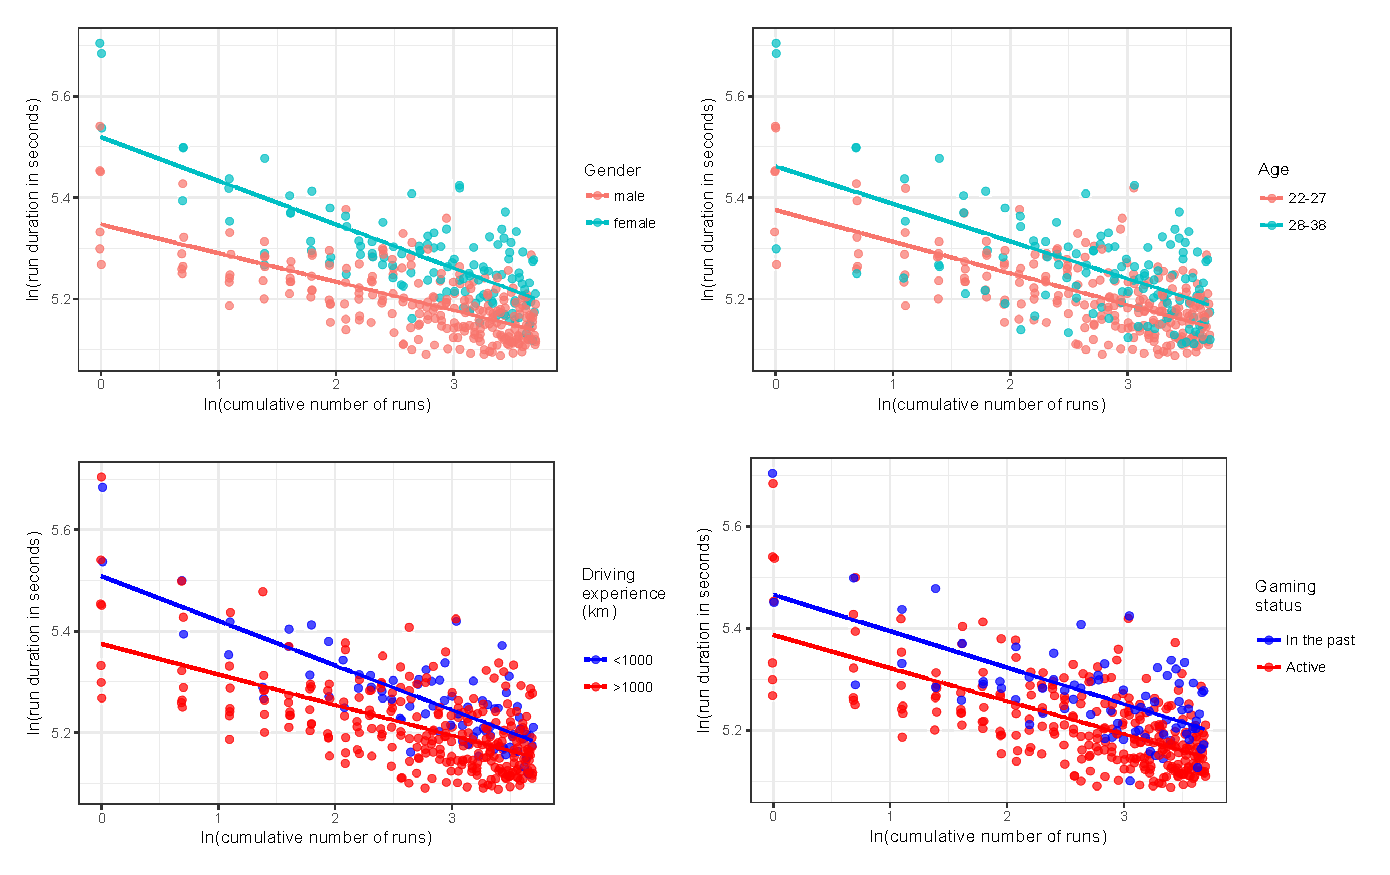
\includegraphics[width=\linewidth]{suppl_learningcurve_groups}
\captionof{figure}{Visualisation of performance data coloured by demographic grouping factors: {\it top-left panel}, gender; {\it top-right panel}, age; {\it lower-left panel}, driving experience; {\it lower-right panel}, gaming experience. Each plot displays log-transformed cumulative trials and trial duration, thus representing a log-log space, where linear regression lines fitted to data subgroups are power law models in linear space.}
\label{fig:supp_LC_groups}
\end{minipage}%



\begin{table}[!h]
\centering
\caption{\label{tab:FluencyAbsorption}Descriptive statistics for fluency of performance and absorption by activity for each participant.}
\begin{tabular}{lllllll}
\hline
           & Participant & Mean & Median & SD   & Min  & Max  \\
\hline
Fluency    &             &      &        &      &      &      \\
           & 1           & 4.93 & 5.00   & .62  & 3.17 & 6.00 \\
           & 2           & 4.90 & 4.83   & .47  & 3.83 & 5.67 \\
           & 3           & 4.90 & 5.00   & .84  & 3.00 & 6.67 \\
           & 4           & 4.10 & 4.00   & .56  & 3.00 & 5.33 \\
           & 5           & 5.15 & 5.50   & 1.01 & 2.67 & 6.50 \\
           & 6           & 5.11 & 5.25   & .92  & 2.83 & 6.50 \\
           & 7           & 4.35 & 4.33   & .58  & 3.17 & 5.50 \\
           & 8           & 4.74 & 5.00   & .92  & 2.50 & 6.33 \\
           & 9           & 5.24 & 5.00   & .86  & 3.33 & 7.00 \\
\hline
Absorption &             &      &        &      &      &      \\
           & 1           & 5.37 & 5.50   & .45  & 4.25 & 6.25 \\
           & 2           & 5.60 & 5.75   & .37  & 5.00 & 6.00 \\
           & 3           & 6.04 & 6.00   & .43  & 5.25 & 6.75 \\
           & 4           & 4.85 & 4.88   & .39  & 4.00 & 5.75 \\
           & 5           & 5.89 & 6.0    & .80  & 3.50 & 7.00 \\
           & 6           & 5.37 & 5.50   & .74  & 3.50 & 6.75 \\
           & 7           & 5.19 & 5.25   & .54  & 4.25 & 6.25 \\
           & 8           & 5.24 & 5.50   & .95  & 3.00 & 6.75 \\
           & 9           & 5.27 & 5.13   & .72  & 4.00 & 6.75 \\
\hline
\end{tabular}
\end{table}

\noindent
\begin{minipage}{\textwidth}
\centering
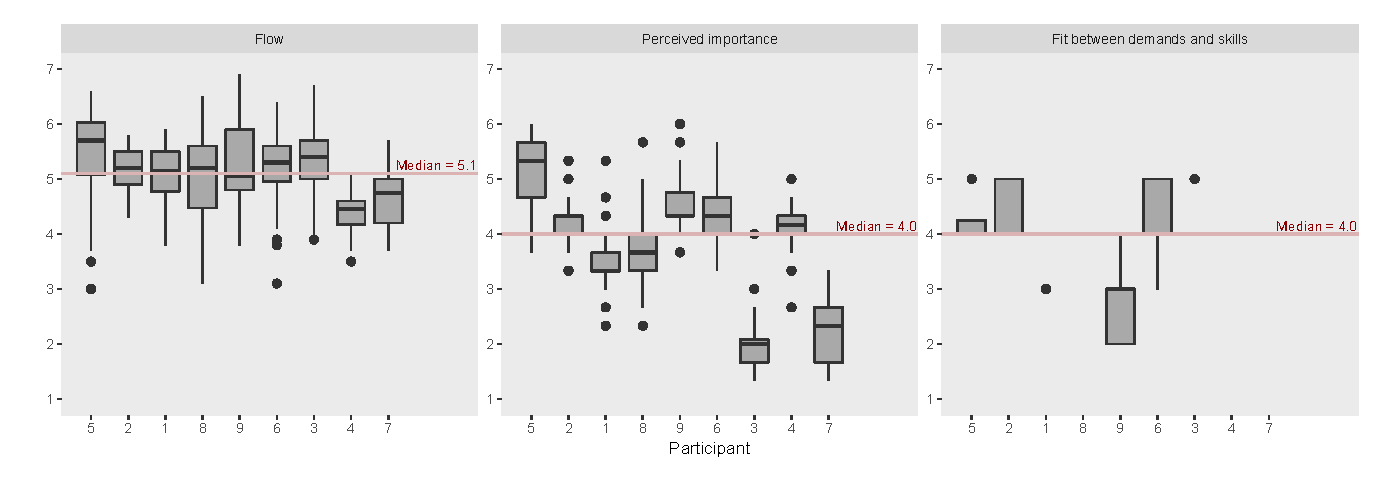
\includegraphics[width=\linewidth]{suppl_fss_boxplots}
\captionof{figure}{Participant-wise boxplots for Flow Short Scale measures, {\it left panel}: Flow (absorption \& fluency), median 5.1, min 3, max 7; {\it center panel}: perceived importance, median 4, min 1, max 6; {\it right panel}: perceived fit of demands and skills, median 4, min 2, max 5. In each plot, boxes are ordered left-to-right by the game performance (mean trial duration) of participants, i.e. from best performer \#5 to worst \#7.}
\label{fig:supp_boxes}
\end{minipage}%


\noindent
\begin{minipage}{\textwidth}
\centering
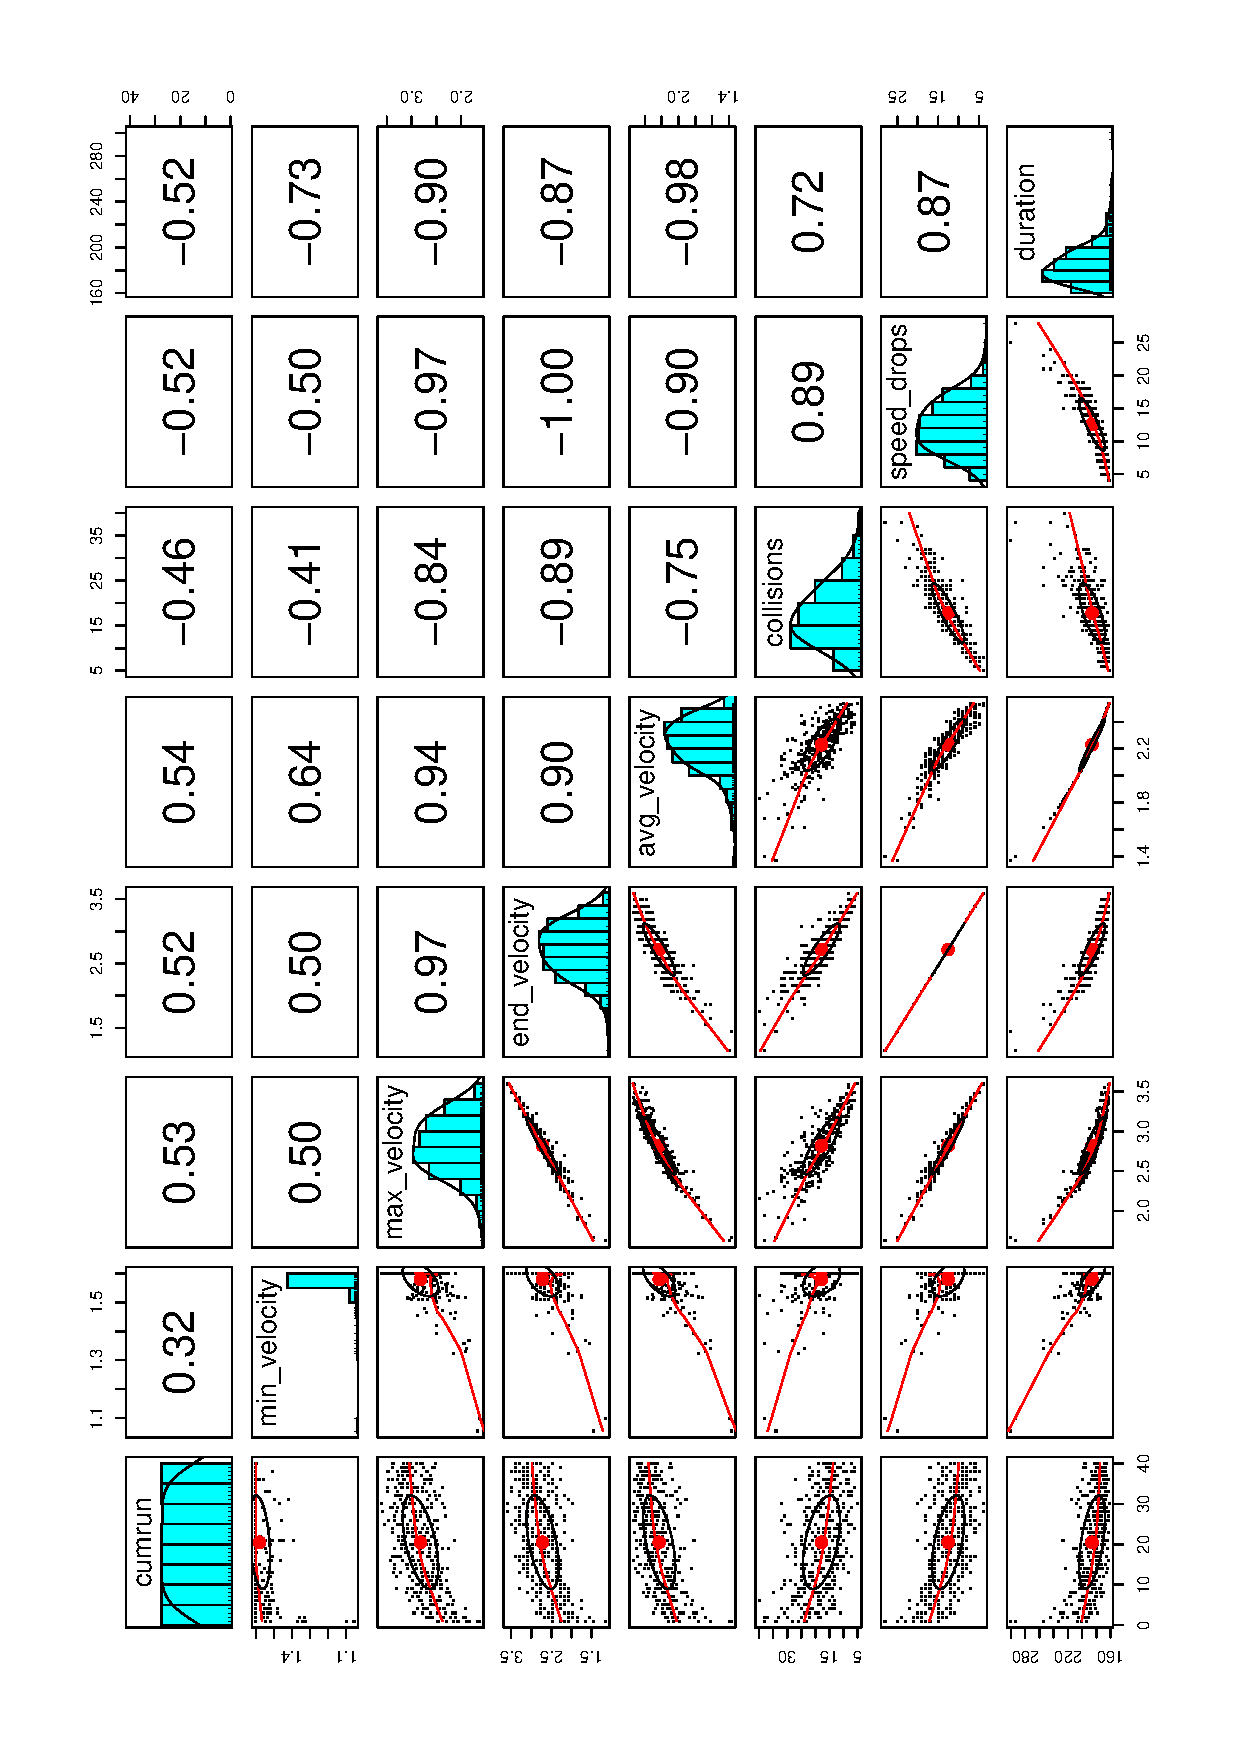
\includegraphics[angle=270,width=\linewidth]{suppl_scattermat}
\captionof{figure}{A scatterplot matrix of game performance measures. The diagonal of the matrix displays distributions (histograms) of each measure. The lower off-diagonal cells contain scatterplots, with loess-smoothed fit, of two measures from the corresponding row and column on the diagonal (panel above on the x-axis; panel to right on y-axis). The upper off-diagonal cells display corresponding Pearson correlation coefficients.}
\label{fig:scatter_matrix}
\end{minipage}

\wineAm{0.5}{1.0}{270}{10cm}{7cm}


\noindent
\begin{minipage}{\textwidth}
\begin{minipage}{.6\textwidth}
\centering
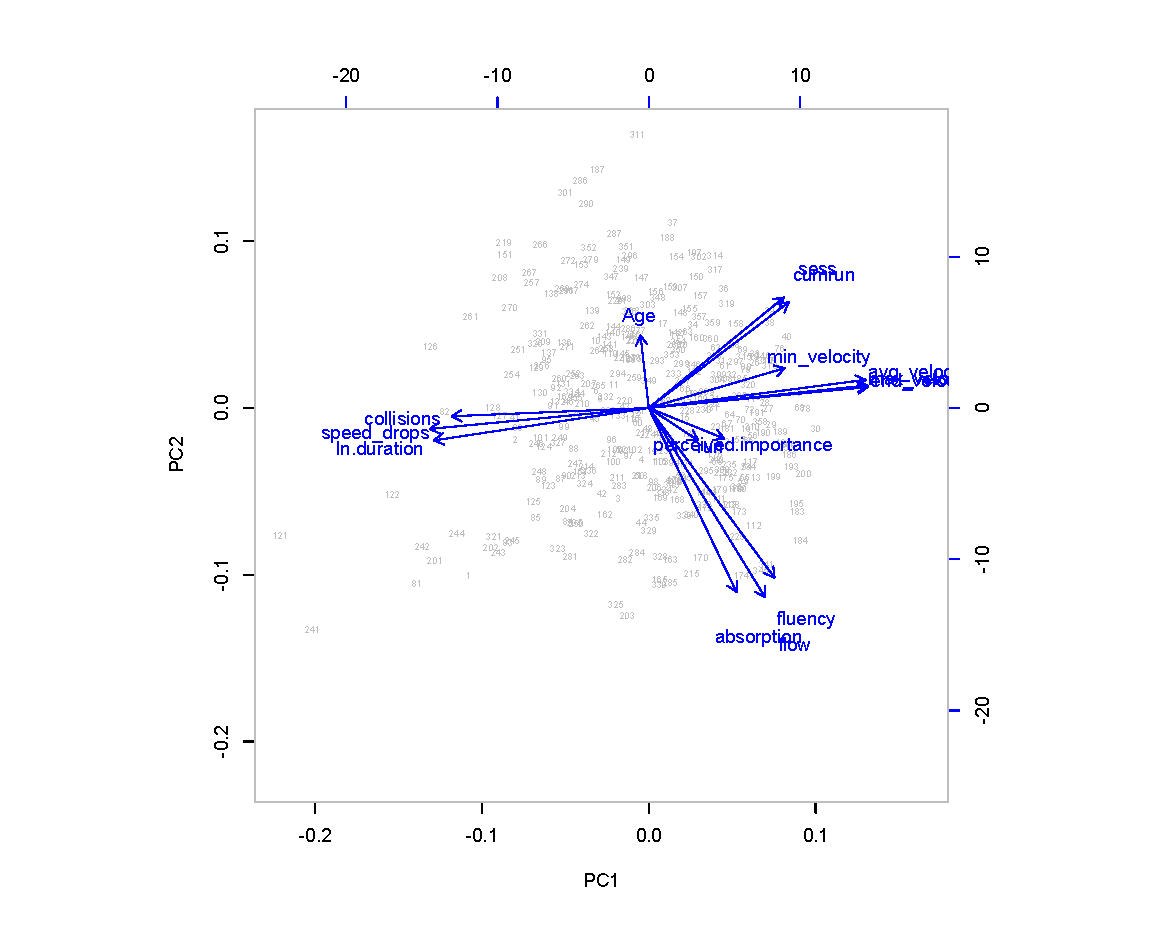
\includegraphics[width=\linewidth]{suppl_pca}
\label{fig:supp_boxes}
\end{minipage}% This must go next to `\end{minipage}`
\begin{minipage}{.4\textwidth}
\begin{tabular}{lll}
{\bf Variable}   &{\bf PC1}&{\bf PC2}\\
\hline
run (trial)      & 0.801  & -0.088 \\
min\_velocity    & 0.221  & 0.109  \\
max\_velocity    & 0.356  & 0.062  \\
end\_velocity    & 0.356  & 0.057  \\
avg\_velocity    & 0.353  & 0.076  \\
collisions       & -0.321 & -0.023 \\
speed\_drops     & -0.356 & -0.057 \\
cumrun (trials)  & 0.228  & 0.289  \\
age              & -0.134 & 0.198  \\
fss\_fluency     & 0.204  & -0.464 \\
fss\_absorption  & 0.143  & -0.502 \\
perc. importance & 0.122  & -0.083 \\
Flow             & 0.189  & -0.517 \\
session          & 0.219  & 0.302  \\
ln.duration      & -0.349 & -0.089
\end{tabular}
\end{minipage}
\captionof{figure}{Summary of principal component analysis results: {\it Left panel} Biplot of principal components (PCs) 1 and 2; {\it Right panel} Component loadings for PC1 and PC2. Notice how Flow total score, and factors absorption and fluency, had distinctly negative loadings on PC2 compared to other variables. Also, Flow scores have almost completely orthogonal relationship to measures of game experience (session number and cumulative number of trials).}
\end{minipage}

\subsection*{Additional Statistical Analyses}

Permutation testing is another way to assess the statistical significance of the results presented in Figures 2A and B in the main text. For each participant, we first obtained their signed residuals from the power law model (see Figure 2A), which we then multiplied by their z-standardized Flow scores and summed across all trials.

This yielded $d_o$ (observed deviation) scores, which have positive values when participants report higher Flow during better-than-predicted trials, {\it or} when they report lower Flow during worse-than-predicted trials. In other words, higher $d_o$ scores reflect better agreement with the hypothesis that {\it participants report more Flow during better-than-predicted trials and vice versa for worse-than-predicted trials}. Thus, for each participant, we define the agreement of the Flow scores with the local performance prediction of the learning curve model using formula~\ref{eq:flowfit}:

\begin{equation}
	\label{eq:flowfit}
	d = \sum_{x=1}^{40} \frac{f_x.(LCy_x - y_x)}{2}
\end{equation}

where $x\in X$ is a trial from the set of all trials for a subject; and at each trial $x$: $y_x$ is the observed performance, $LCy_x$ is the performance value predicted by the learning curve model, and $f_x$ is the standardised Flow score.

Next, we randomly permuted (over 10000 iterations) standardized Flow scores for each 40 trials for each participant and calculated a $d_p$ (permuted deviation) score for each iteration. Finally, we obtained the distribution (histogram) of the permuted $d_p$ values and computed the probability that the observed $d_o$ values came from this distribution. For participants 1-9, these probabilities were $<$0.001, 0.012, 0.076, $<$0.001, $<$0.001, $<$0.001, 0.025, 0.002, and $<$0.001, respectively. See Fig.~\ref{fig:suppl_permute_cogcar} for participant-wise permuted histograms of $d_p$ values, with a vertical line marking the observed $d_o$ value for each participant.

%\noindent
\begin{figure}[!h]%{\textwidth}
\centering
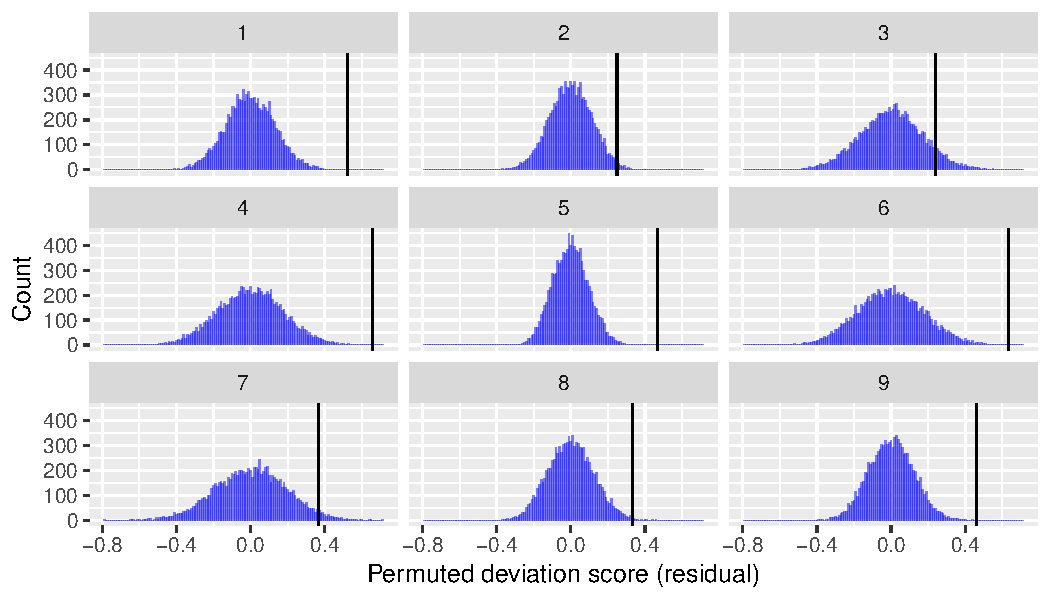
\includegraphics[width=\linewidth]{suppl_permute_cogcar}
\caption{Participant-wise histograms of randomly-permuted deviation scores, with the actual observed deviation score marked as a black line. Here, we can see that the observed relationship between local Flow and performance is very unlikely to have been generated by a random process, even for those participants whose observed $d_o$ value is closer to the random mean.}
\label{fig:suppl_permute_cogcar}
\end{figure}

Finally, we compared the model fit criteria between the power law model (reported in the main text) and an exponential curve model as approximations of learning in the task. The exponential curve model had AIC and BIC values of -992.2 and -968.9, respectively, and a marginal pseudo-$R^2$ value of .289 ~\cite{nakagawa2013general}. The corresponding values for the power law model were -1118.6, -1095.3, and .397. Thus, while both models had a good fit, the power law model was slightly better across all fit indices. See Fig.~\ref{fig:suppl_exp_law} for participant-wise data on the exponential curve model (transformed into linear space).


\noindent
\begin{minipage}{\textwidth}
\centering
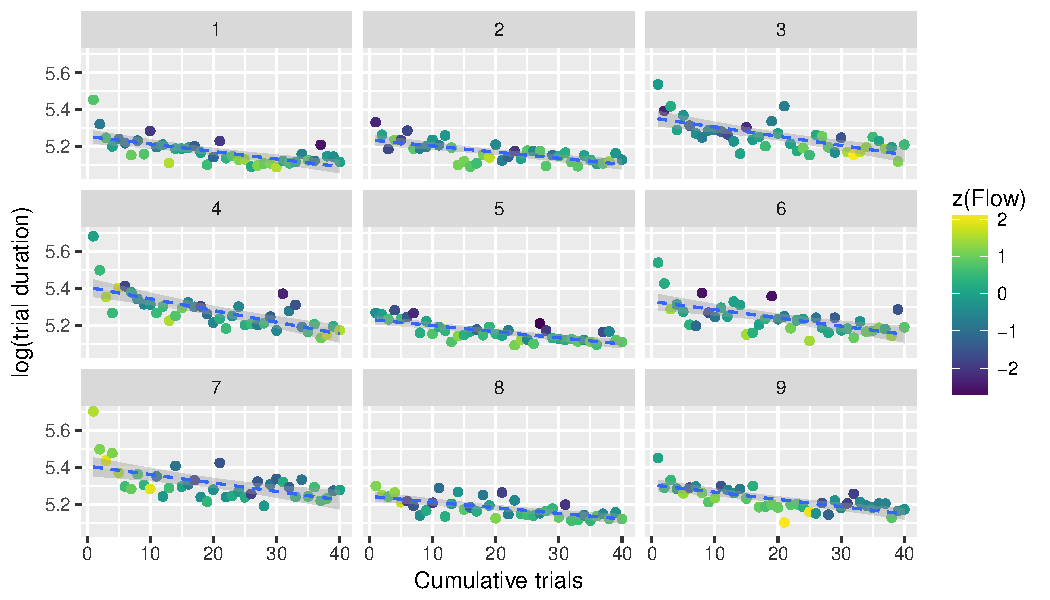
\includegraphics[width=\linewidth]{suppl_explaw_anon}
\captionof{figure}{Participant-wise data showing logarithm-transformed performance and Flow self-reports in the speeded steering task. Ordinate shows log-duration of trials, abscissa shows raw cumulative trial count. Dashed blue lines fitted to the data are exponential law learning curves, which transform to linear when the dependent variable is log-transformed}
\label{fig:suppl_exp_law}
\end{minipage}


\end{document}
